%%%%%%%%%%%%%%%%%%%%%%%%%%%%%%%%%%%%%%%%%%%%%%%%%%%%%%%%%%%%%%%%%%%%%%
% LaTeX Template: Beamer arrows
%
% Source: http://www.texample.net/
% Feel free to distribute this template, but please keep the
% referal to TeXample.net.
% Date: Nov 2006
% 
%%%%%%%%%%%%%%%%%%%%%%%%%%%%%%%%%%%%%%%%%%%%%%%%%%%%%%%%%%%%%%%%%%%%%%


\documentclass{beamer} %
\usetheme{CambridgeUS}
\usepackage[latin1]{inputenc}
\usefonttheme{professionalfonts}
\usepackage{times}
\usepackage{tikz}
\usepackage{amsmath}
\usepackage{graphicx}
\usepackage{url}
\usepackage{array} % needed for \arraybackslash
\usepackage{adjustbox} % for \adjincludegraphics
\usepackage{subcaption}
\usepackage{verbatim}
\usetikzlibrary{arrows,shapes}
\usepackage[absolute,overlay]{textpos}
\usepackage{listings}
\usepackage{pdfcomment}
\captionsetup{compatibility=false}

\newcommand{\pdfnote}[1]{\marginnote{\pdfcomment[icon=note]{#1}}}

%alex special colors
\usepackage{color}

\definecolor{alexred}{RGB}{239,138,98}
\definecolor{alexgreen}{RGB}{145,207,96}
\definecolor{alexblue}{RGB}{103,169,207}


% gets rid of bottom navigation bars
%\setbeamertemplate{footline}[page number]{}

% gets rid of navigation symbols
\setbeamertemplate{navigation symbols}{}

% add figures numbering
\setbeamertemplate{caption}[numbered]


%source information

\newcommand{\source}[1]{\begin{textblock*}{3.9cm}(8.8cm,8.8cm)
		\begin{beamercolorbox}[ht=0.3cm,right]{framesource}
			\usebeamerfont{framesource}\usebeamercolor[fg]{framesource} \tiny Source: {#1}
		\end{beamercolorbox}
\end{textblock*}}

\begin{document}

\author{A Peltzer \& J Neukamm}
%\title{Oberseminar Integrative Transcriptomics}
\title[mitoBenchDB]{mitoBench \& mitoDB}
\institute[IT/INA/MPI-SHH]{Integrative Transcriptomics, University of Tuebingen\\
     INA, WG: Archaeo- and Paleogenetics, University of Tuebingen \\
     Max-Planck Institute for the Science of Human History, Jena}
\date{February $23^{\text{rd}}$, 2017}
\titlegraphic{
\includegraphics[width=2cm]{images/mpi-logo.png}\hspace*{3cm}~%
              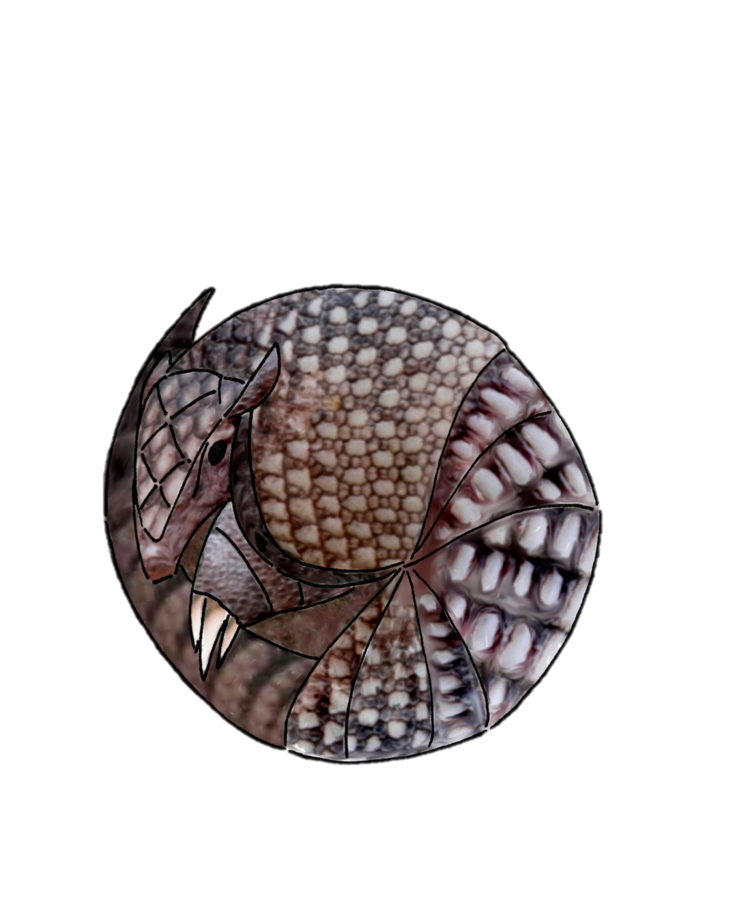
\includegraphics[width=2cm]{images/Pali_Freigestellt2.png}\hspace*{2.5cm}~%
			  
\includegraphics[width=2cm]{images/it-logo.png}}
\setbeamertemplate{footline}[page number]{}

\maketitle

\begin{frame}
\frametitle{Overview}
\begin{itemize}
\item Introduction \& Motivation
\item mitoBench
\item mitoDB
\item Outlook
\end{itemize}
\end{frame}

\begin{frame}
\frametitle{Introduction: Overview}
\begin{tabular}{p{.3\textwidth} p{.7\textwidth}}
\adjincludegraphics[width=1.0\linewidth,valign=t]{images_mummies/2016-10-06_Figure1.png}
&
\adjincludegraphics[width=1.0\linewidth,valign=t]{images_mummies/abusir_natGeo.png}\source{National Geographic, June 2016}
\end{tabular}
\vfill\textbf{Intent:} Study population history of Egypt
\end{frame}

\begin{frame}
\frametitle{Introduction: Overview}
\begin{itemize}
\item After mitochondrial (bead) capture: $90$ individuals, authenticated (damage $10-20\%$), endogenous DNA between $14-60\%$
\item Low Contamination (threshold: $<3\%$) 
\end{itemize}
\end{frame}

\begin{frame}
\frametitle{Introduction: Overview}
\begin{itemize}
\item Sequence based analysis: Calculate population differentiation (e.g. $F_{st}$)
\item Haplotype based analysis: Determine maternal Haplogroups (e.g. with HaploGrep2\footnote{Weissensteiner, Hansi, et al. \textit{"HaploGrep 2: mitochondrial haplogroup classification in the era of high-throughput sequencing."} Nucleic acids research (2016)})
\end{itemize}
\end{frame}

\begin{frame}
\frametitle{Introduction: Overview}
\begin{itemize}
\item What do we need? \pause
\begin{itemize}
\item Comparison data: Both sequence information and haplogroups \pause
\item Several file formats for downstream tools: ARP, XLSX, FastA, \ldots
\end{itemize}
\end{itemize}
\end{frame}

\begin{frame}
\frametitle{Mitochondrial Genomics: Current status}
\begin{itemize}
\item Not so much a problem of getting the data
\pause
\begin{itemize}
\item Lots of people work on this (dozens of labs)\pause
\item Fairly cheap per genome - generate more data if you need more (if samples are available) 
\end{itemize}
\end{itemize}
\end{frame}

\begin{frame}
\frametitle{Mitochondrial Genomics: Current status}
\begin{center}
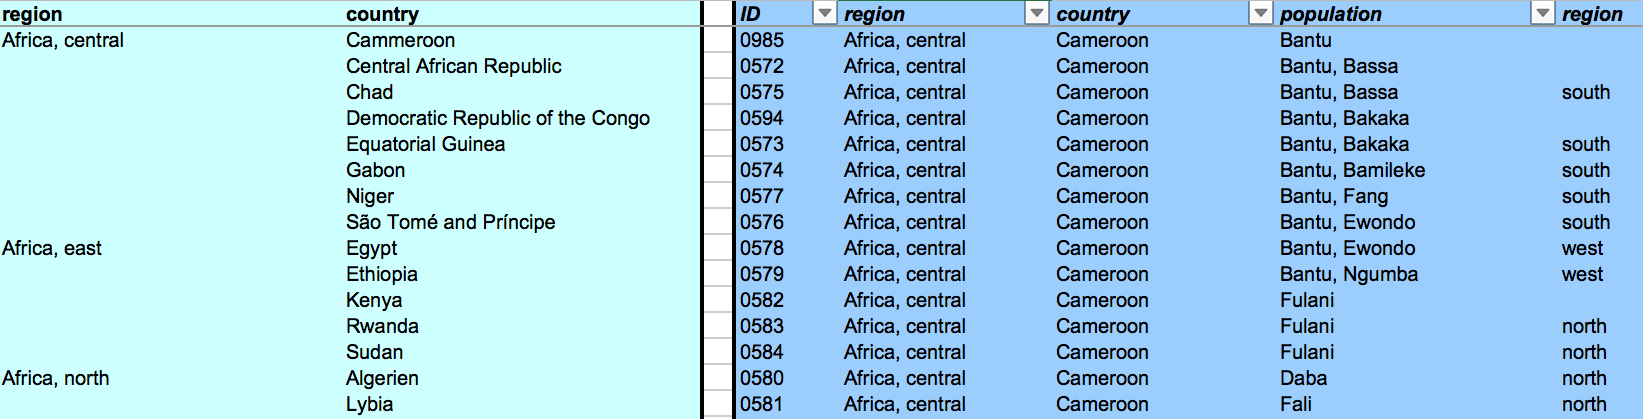
\includegraphics[scale=0.7]{images_mummies/excel_DB.png} \source{Previous internal data source, credits to A Sz\'{e}cs\'{e}nyi-Nagy, G Brandt, W Haak and others}
\end{center}
\end{frame}

\begin{frame}
\frametitle{Mitochondrial Genomics: Current status}
\begin{itemize}
\item More a problem of what to do with it ... \pause
\begin{itemize}
\item Manual conversions (e.g. from FastA to ARP, ...)\pause
\item Collections are kept private (though publicly available data) - room for collaborative improvements
\item Lots of potential for error: Copy \& Paste errors, inconsistent data sources, citing papers is difficult (e.g. where was this sample published again?)
\end{itemize}
\end{itemize}
\end{frame}

\begin{frame}
\frametitle{mitoBench: Introduction}
\begin{flushright}
	
\includegraphics[width=0.3\textwidth]{imagesBench/mitoBenchLogo.jpg}
\end{flushright}
Idea: Mitochondrial Workbench
	\begin{itemize}
		\item Collect mitochondrial data \pause
    	\item Ease file handling and file conversion \pause
        \item Combine, manipulate and visualize MT data
	\end{itemize}

\end{frame}

\begin{frame} 
\frametitle{mitoBench: Workflow}
\begin{center}
	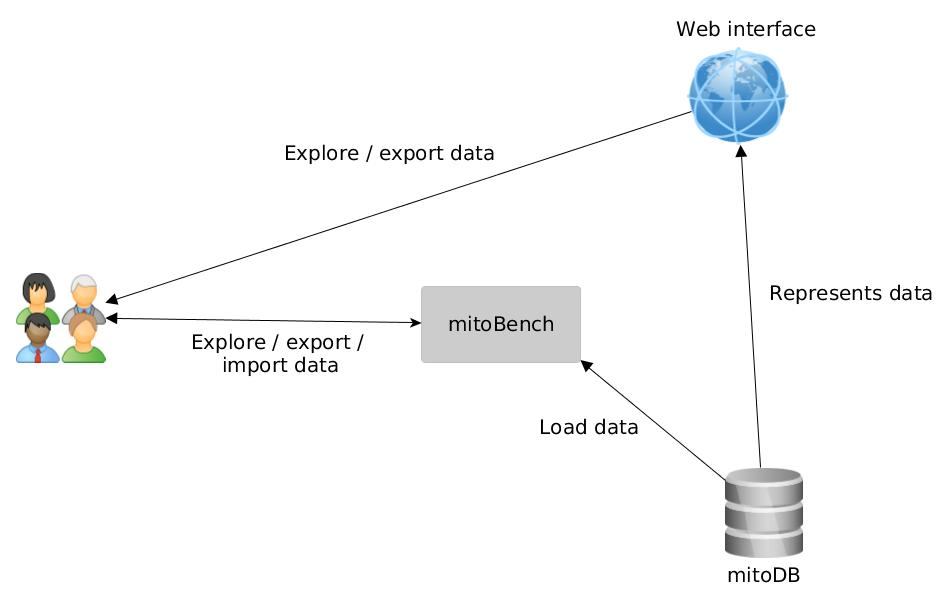
\includegraphics[width=0.7\textwidth]{imagesBench/workflow_yed.jpg}
	\end{center}
\end{frame}

\begin{frame}
	\frametitle{mitoBench: Main view}
		\begin{center}
			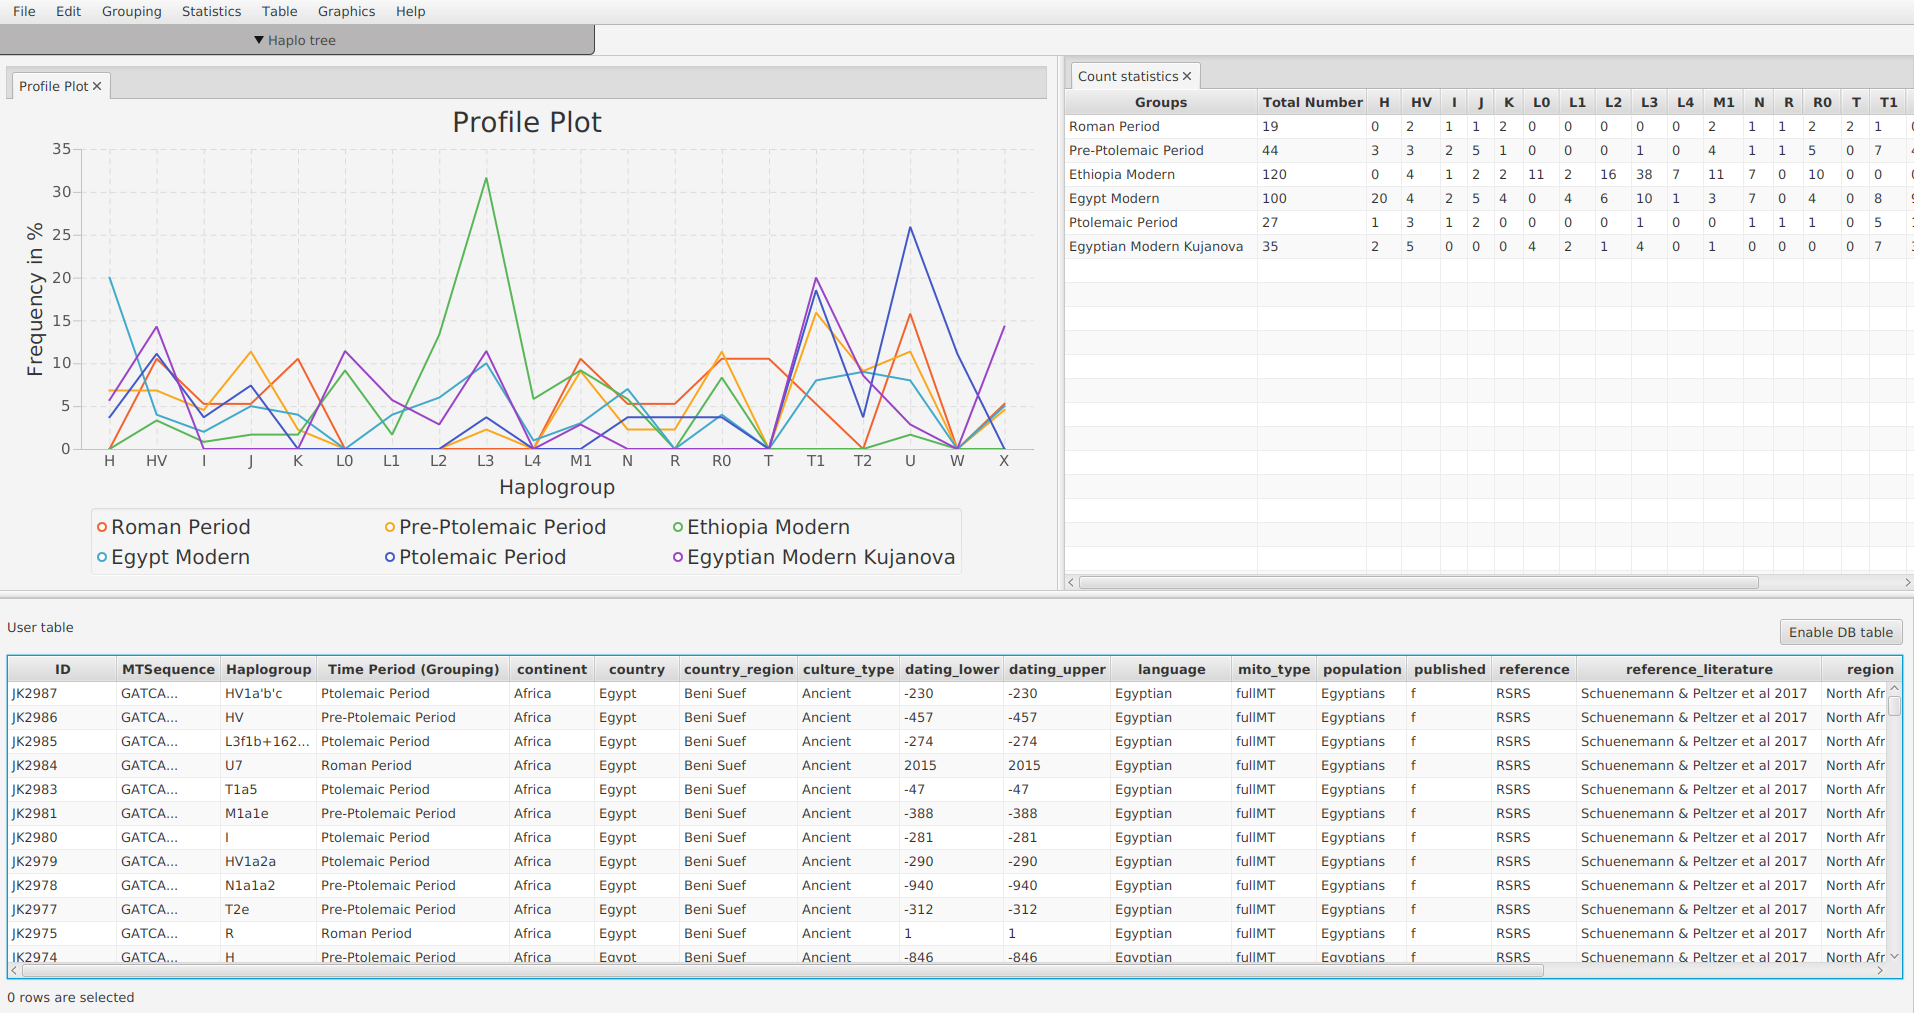
\includegraphics[width=1.0\textwidth]{imagesBench/main.png}
		\end{center}
\end{frame}

\begin{frame}
	\frametitle{mitoBench: Main view}
	\begin{center}
		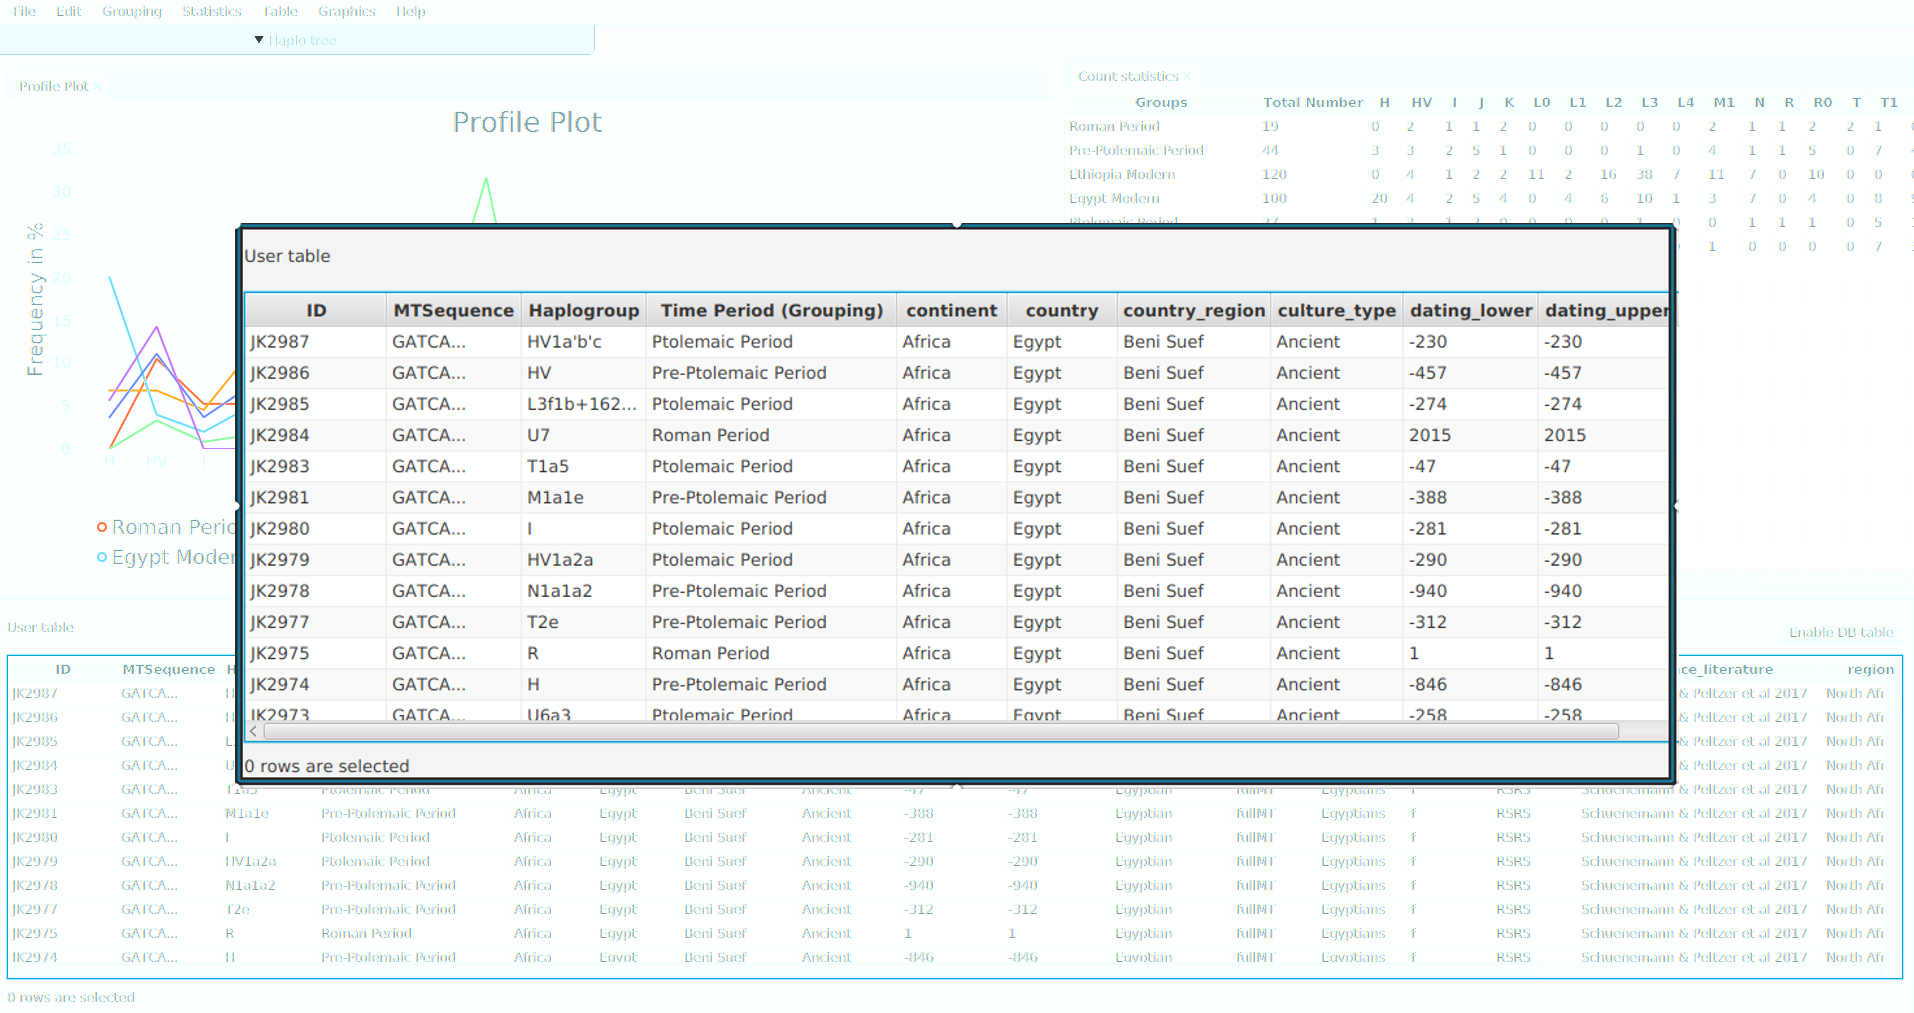
\includegraphics[width=1.0\textwidth]{imagesBench/main_table2.png}
	\end{center}
\end{frame}

\begin{frame}
	\frametitle{mitoBench: Main view}
	\begin{center}
		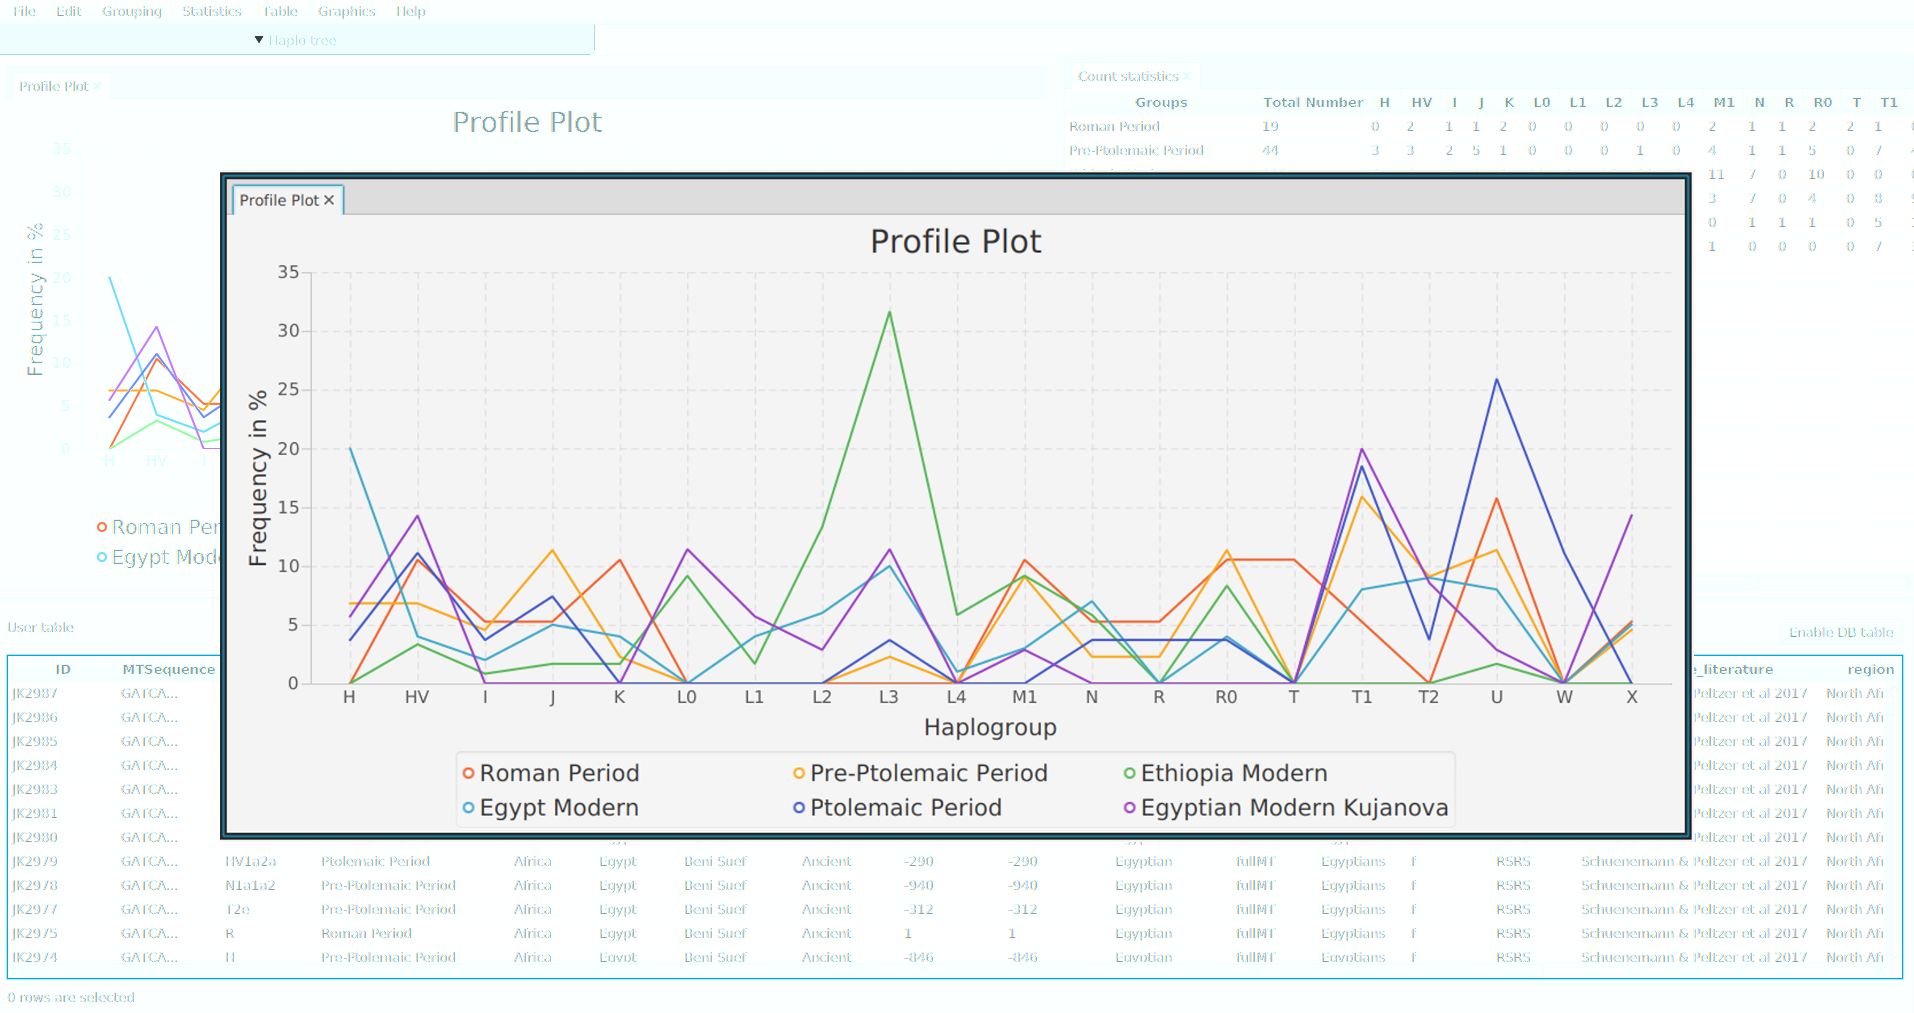
\includegraphics[width=1.0\textwidth]{imagesBench/main_plot2.png}
	\end{center}
\end{frame}

\begin{frame}
	\frametitle{mitoBench: Main view}
	\begin{center}
		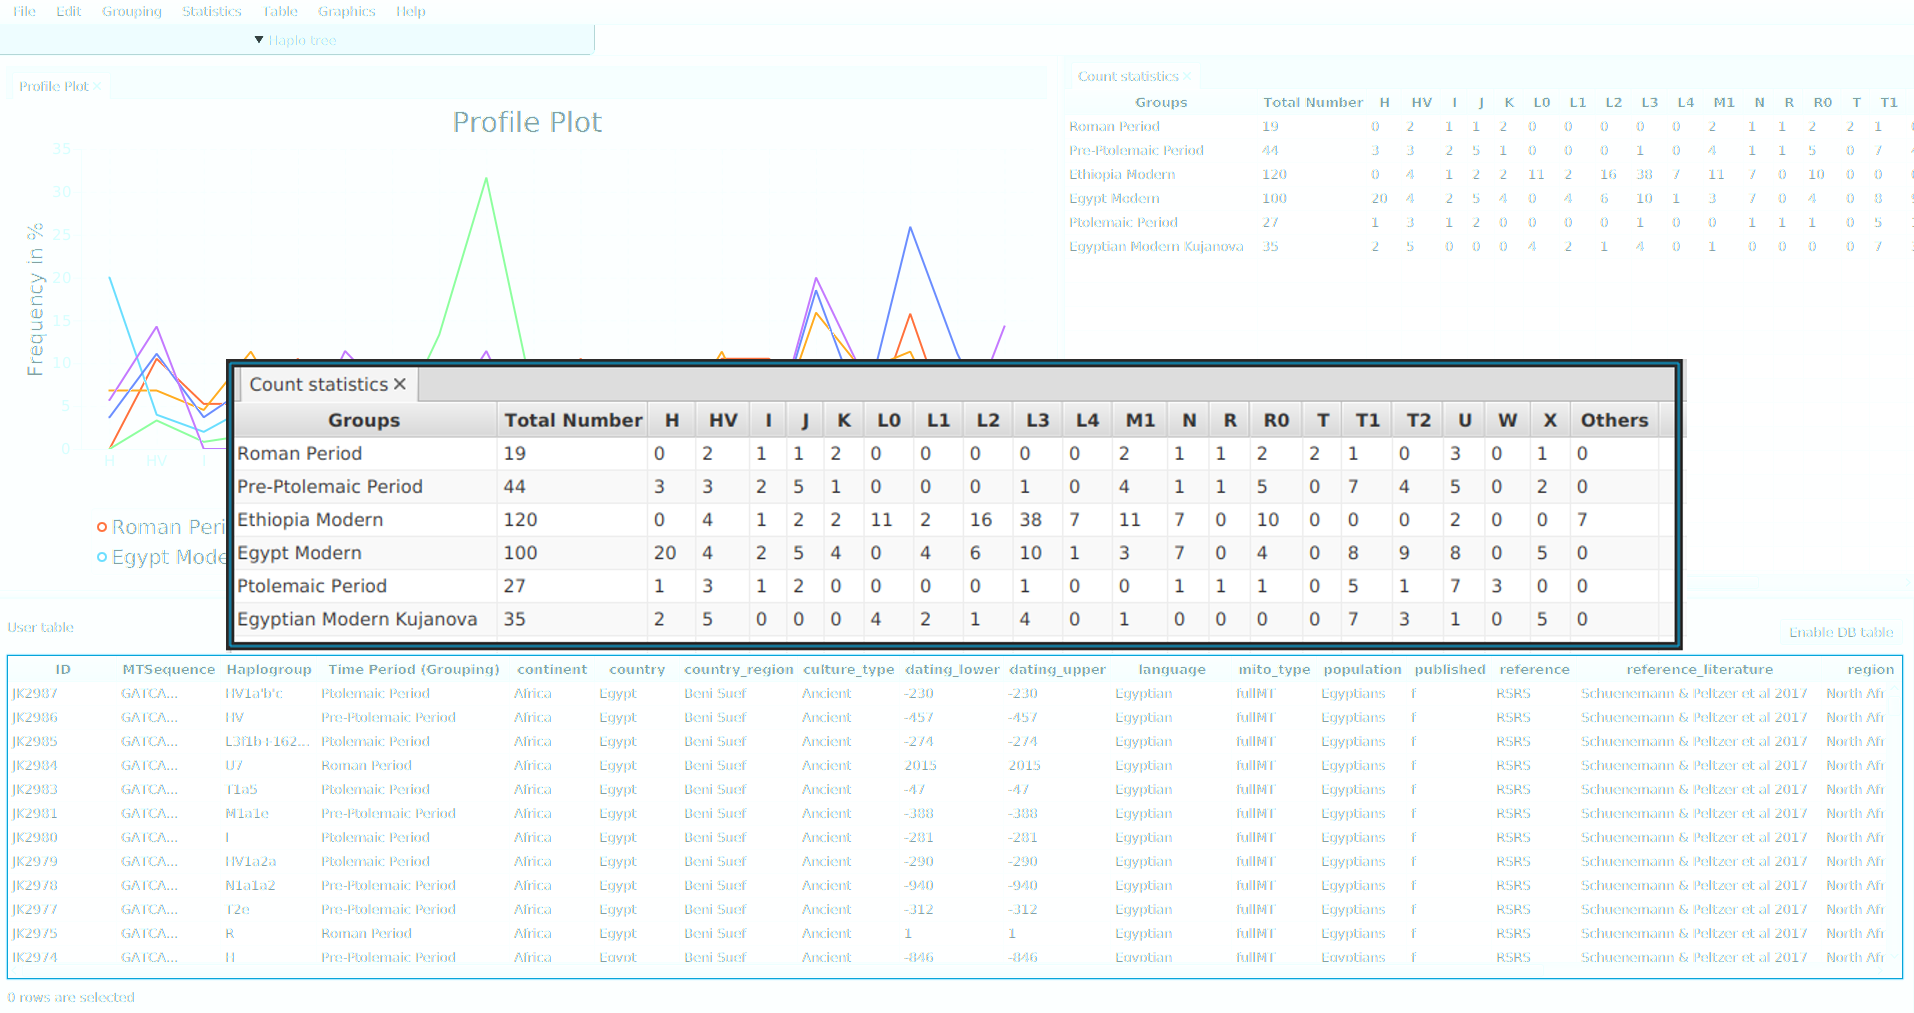
\includegraphics[width=1.0\textwidth]{imagesBench/main_stats2.png}
	\end{center}
\end{frame}

\begin{frame}
\frametitle{mitoBench: Data import and conversion}
Accepted file formats
\begin{itemize}
\item (Multi-) FastA \pause
\item ARP (Arlequin format)\footnote{Excoffier, Laurent, and Heidi EL Lischer. \textit{"Arlequin suite ver 3.5: a new series of programs to perform population genetics analyses under Linux and Windows."} Molecular ecology resources 10.3 (2010): 564-567.} \pause
\item HSD (Haplogrep 2 format) \pause
\item Excel file \pause
\item Generic formats (e.g. dating information, tsv/csv format) 
\end{itemize}
\end{frame}

\begin{frame}
\frametitle{mitoBench: Data import and conversion}
Import from database
\begin{itemize}
	\item Connect to mitoDB via mitoBench \pause
	\item Specify query \pause
    \item Add data to user table
\end{itemize}
\end{frame}

\begin{frame}
	\frametitle{mitoBench: Data import and conversion (Mummies)}
	\begin{itemize}
		\item Load sequences (via fasta file)
	\end{itemize}
	\begin{center}
		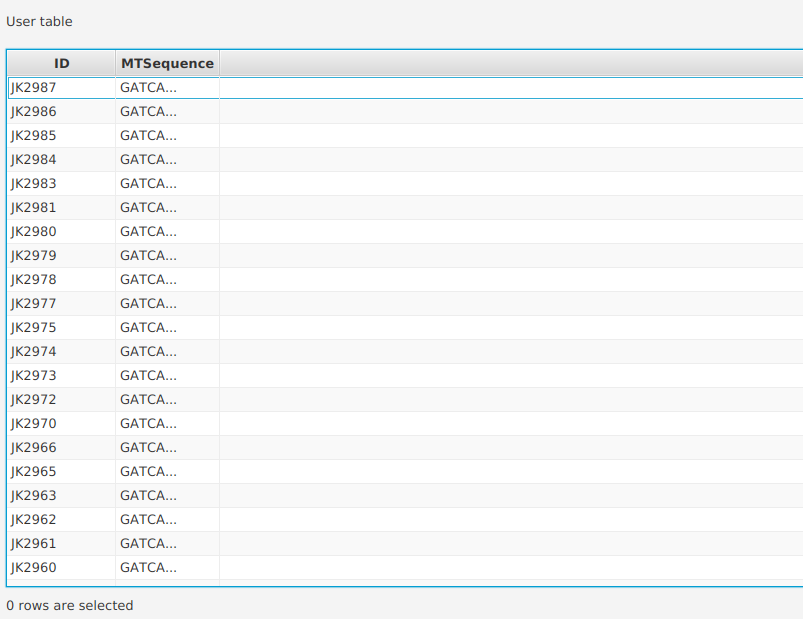
\includegraphics[width=0.7\textwidth]{imagesBench/load_Fasta.png}
	\end{center}
\end{frame}


\begin{frame}
	\frametitle{mitoBench: Data import and conversion (Mummies)}
	\begin{itemize}
		\item Load Haplogroups (via hsd file)
	\end{itemize}
	\begin{center}
		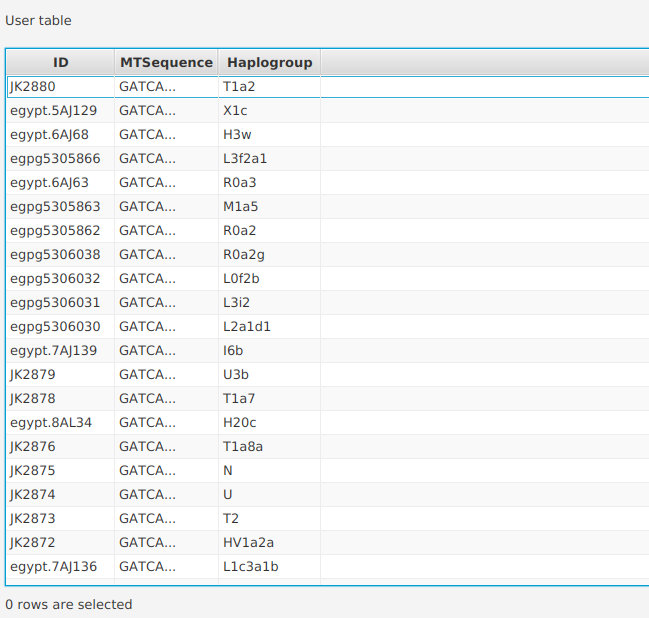
\includegraphics[width=0.6\textwidth]{imagesBench/load_HG.png}
	\end{center}
\end{frame}



\begin{frame}
	\frametitle{mitoBench: Data import and conversion (Mummies)}
	\begin{itemize}
		\item Load generic file (via tsv file)
	\end{itemize}
	\begin{center}
		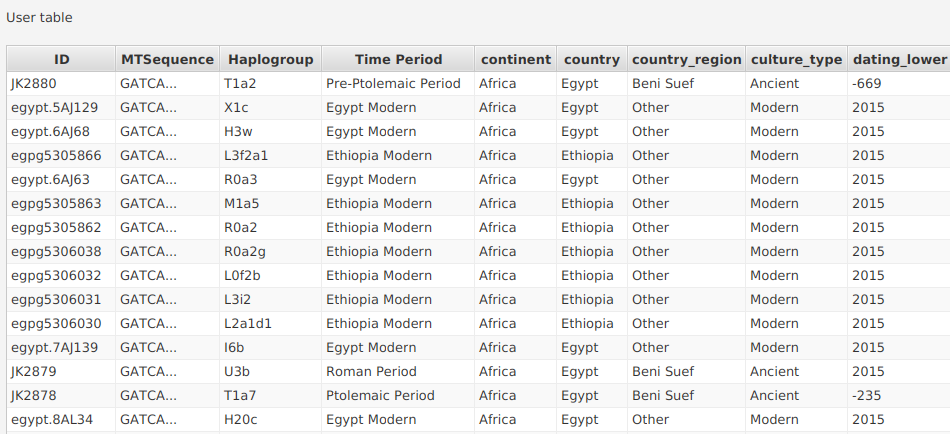
\includegraphics[width=0.9\textwidth]{imagesBench/load_generic.png}
	\end{center}
\end{frame}

\begin{frame}
	\frametitle{mitoBench: Data representation}
	\begin{itemize}
		\item Data represented in table format\pause
		\item Merging data in a single table
	\end{itemize}
%	\begin{center}
%		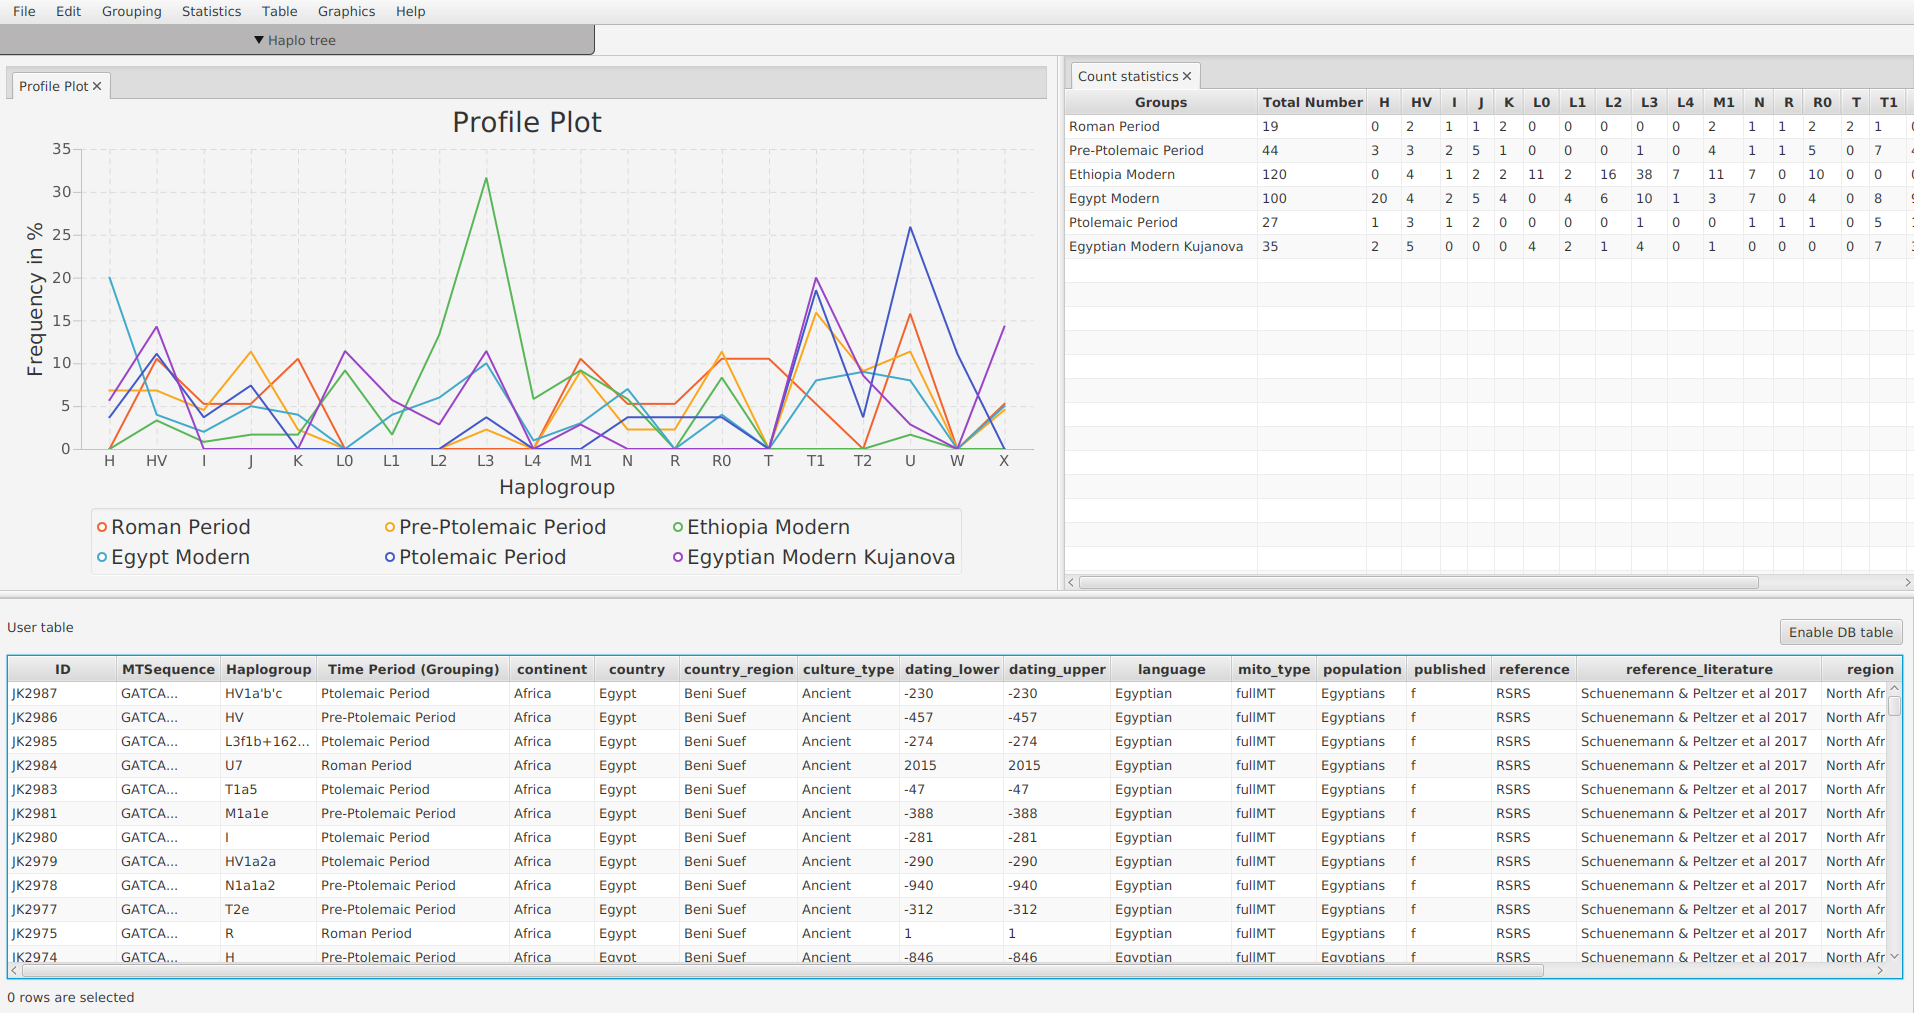
\includegraphics[width=0.9\textwidth]{imagesBench/main.jpg}
%	\end{center}
\end{frame}

\begin{frame}
	\frametitle{mitoBench: Data grouping}
	\begin{itemize}
		\item interested in behavior of different groups\\
		 $\rightarrow$ Group data by feature\pause
		\item internal grouping (columns not sorted)
	\end{itemize}
\end{frame}



\begin{frame}
	\frametitle{mitoBench: Data grouping}
	User-specified groups
	\begin{center}
		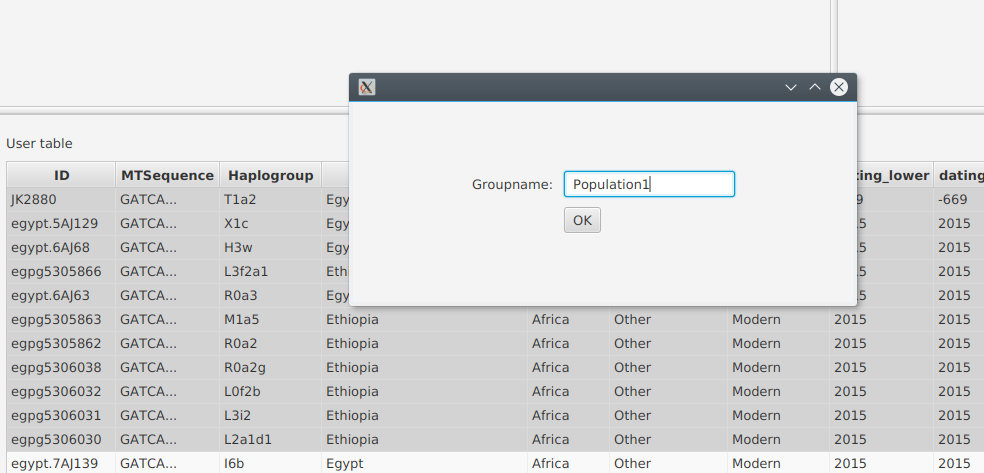
\includegraphics[scale=0.45]{imagesBench/group_user.png}
	\end{center}
\end{frame}



\begin{frame}
\frametitle{mitoBench: Data grouping}
Groups by column
\begin{center}
	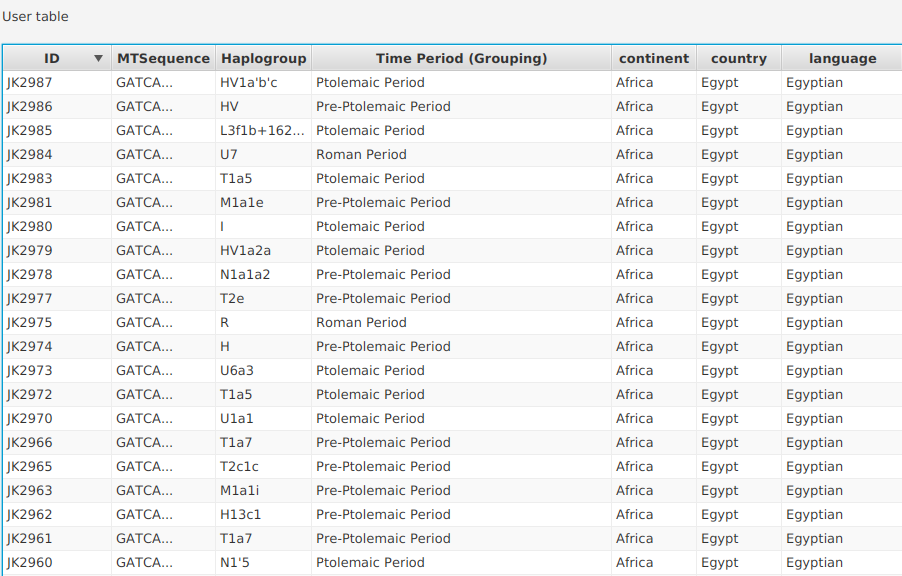
\includegraphics[scale=0.4]{imagesBench/grouping_by_column.png}
\end{center}
\end{frame}




\begin{frame}
\frametitle{mitoBench: Haplotype filtering}

\centering
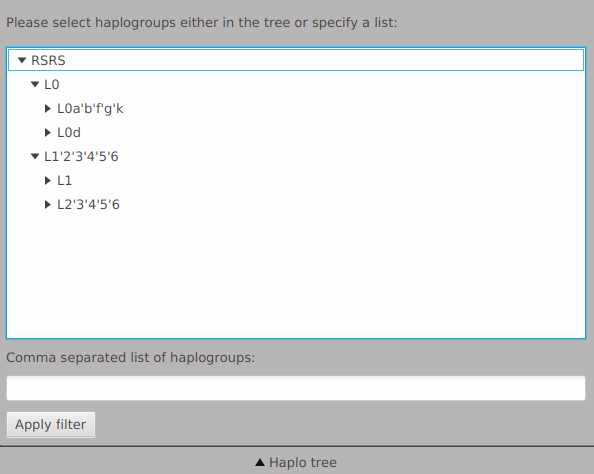
\includegraphics[width=0.45\textwidth]{imagesBench/phylotree.png}

\begin{itemize}
	\item Phylotree\footnotemark embedded into mitoBench \pause
	\item Multiple selection possible \pause
	\item Hierarchical tree-based Haplotype filtering 
\end{itemize}
\bigskip

\footnotetext{van Oven M, Kayser M. 2009. Updated comprehensive phylogenetic tree of global human mitochondrial DNA variation.\textit{Hum Mutat} 30(2):E386-E394. \url{http://www.phylotree.org}.doi:10.1002/humu.20921}


\end{frame}


\begin{frame}
\frametitle{mitoBench: Current visualization methods}
\begin{center}
	\includegraphics[width=\textwidth]{imagesBench/barchart.png}
	\end{center}
\end{frame}



\begin{frame}
\frametitle{mitoBench: Current visualization methods}
\begin{center}
	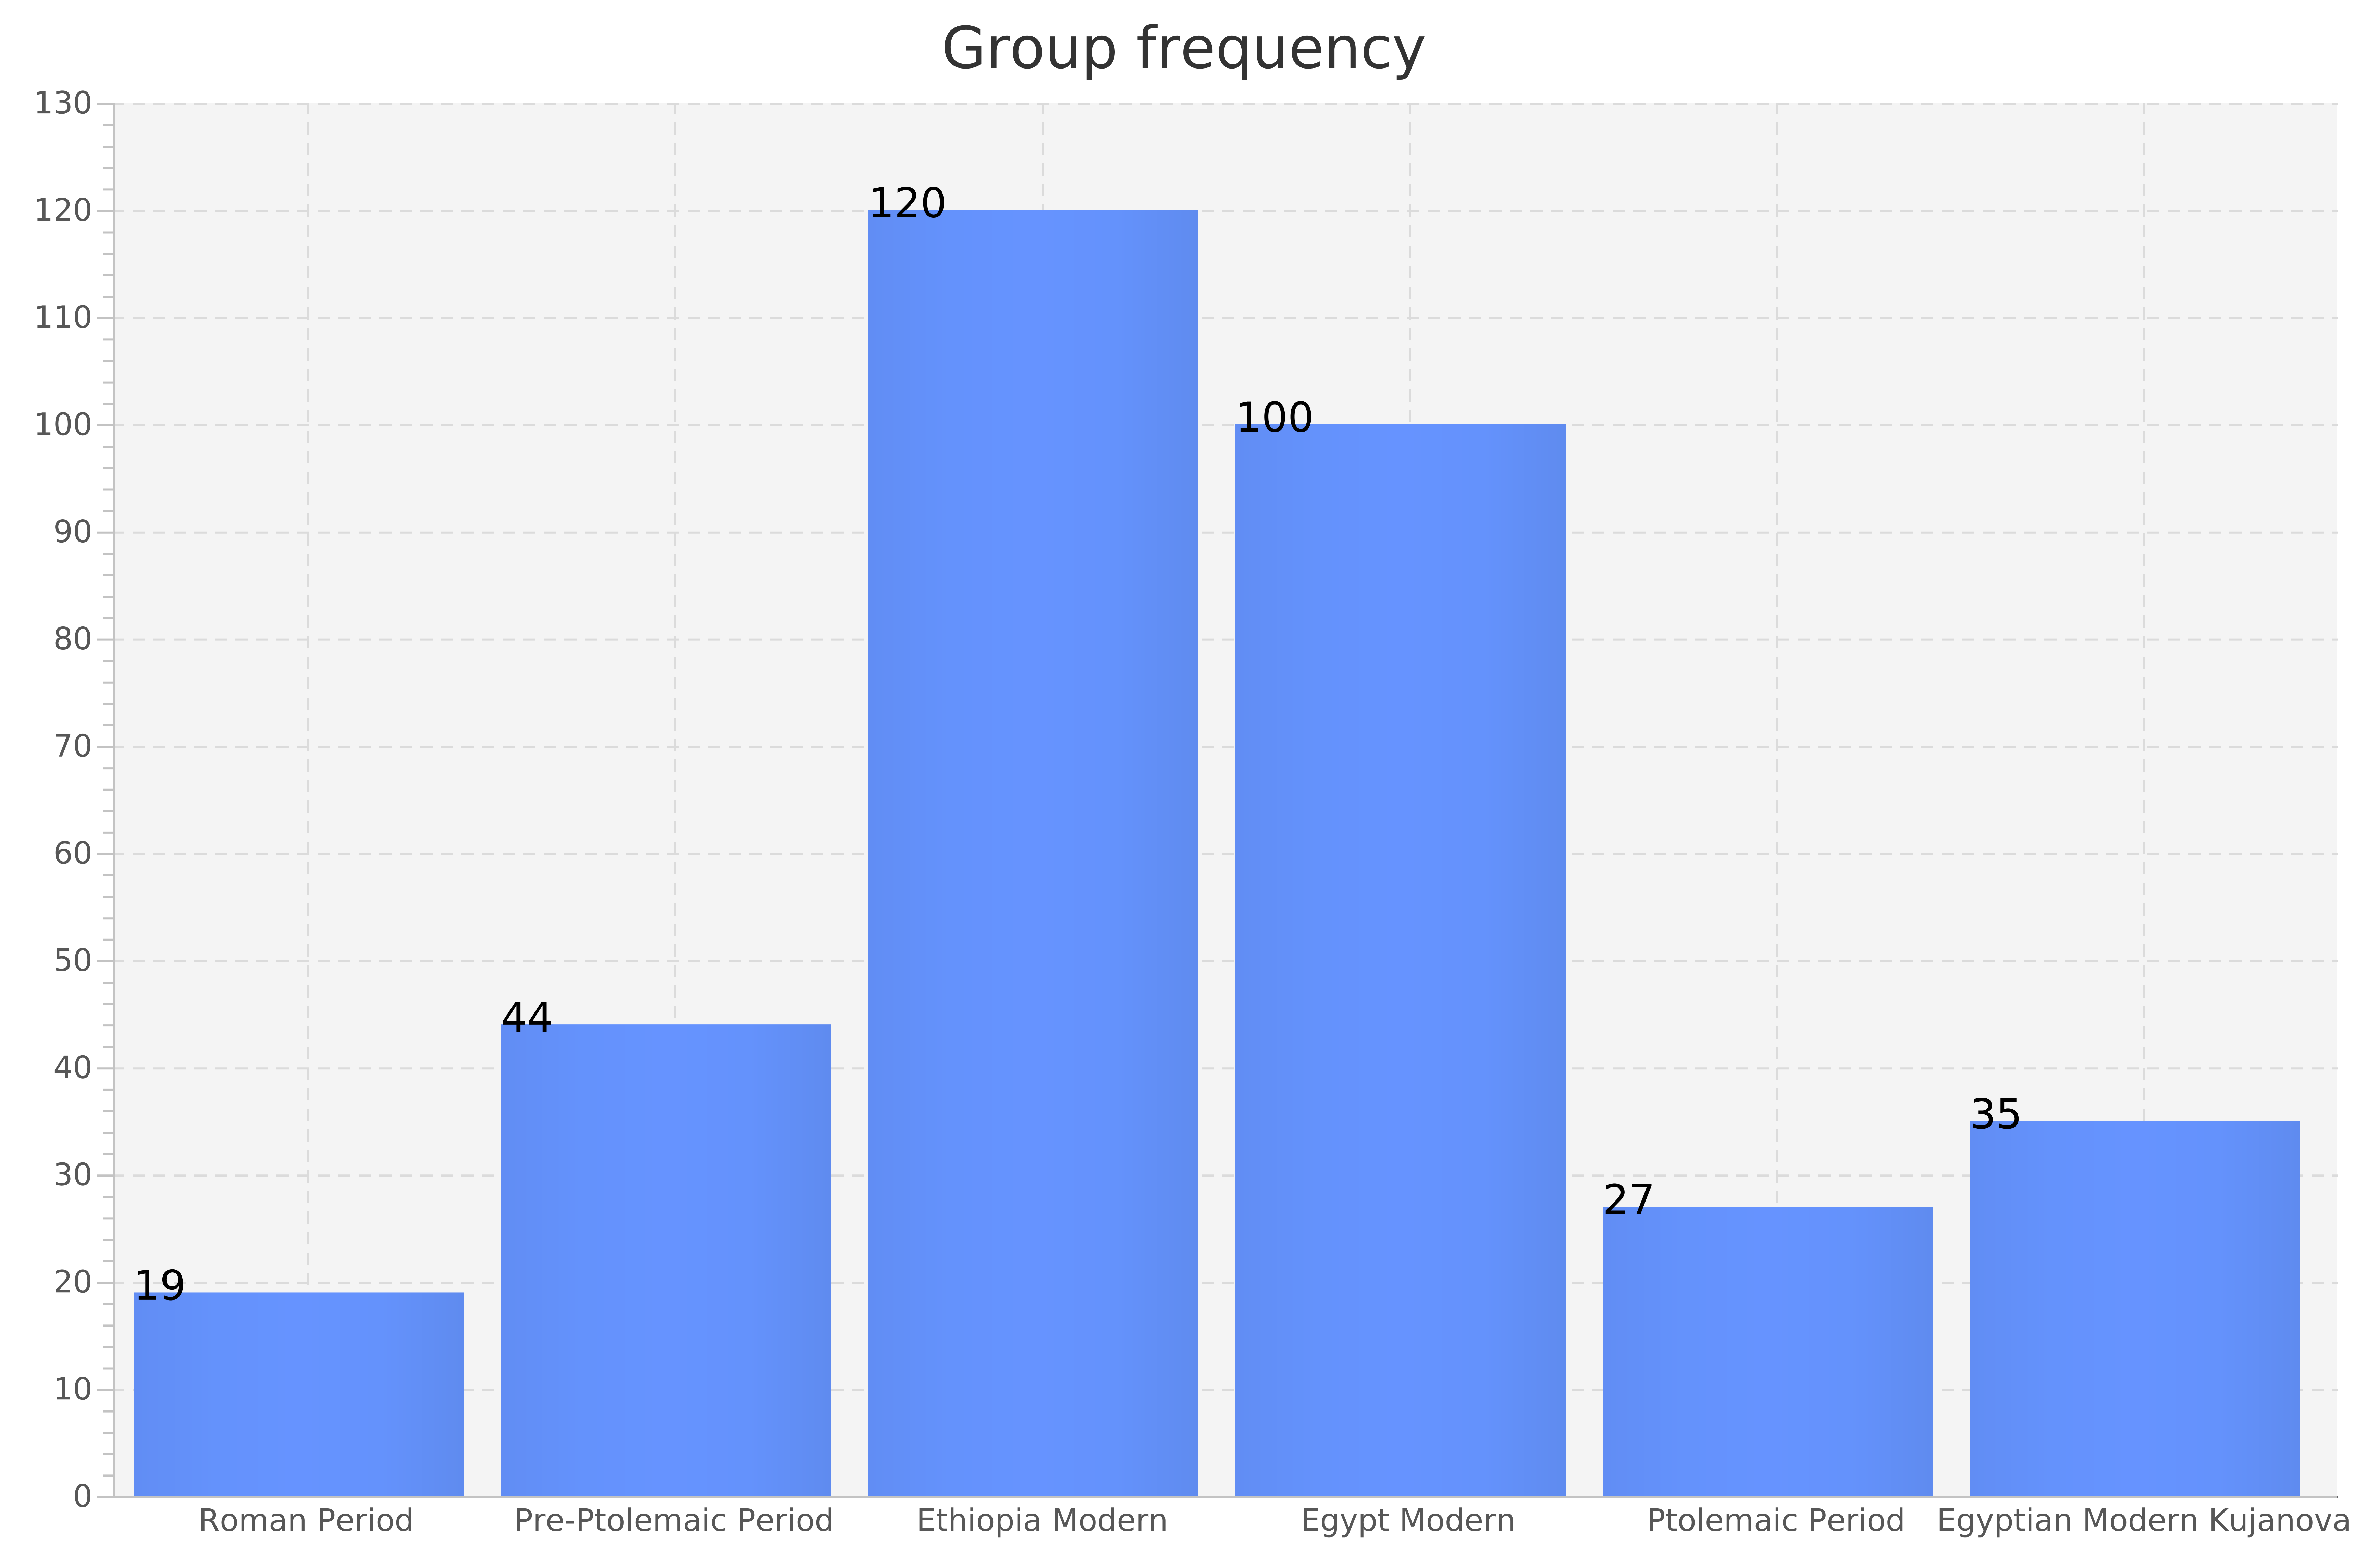
\includegraphics[width=0.7\textwidth]{imagesBench/barchart_group.png}
	\end{center}
\end{frame}



\begin{frame}
	\frametitle{mitobench: Current visualization methods}
	\begin{center}
		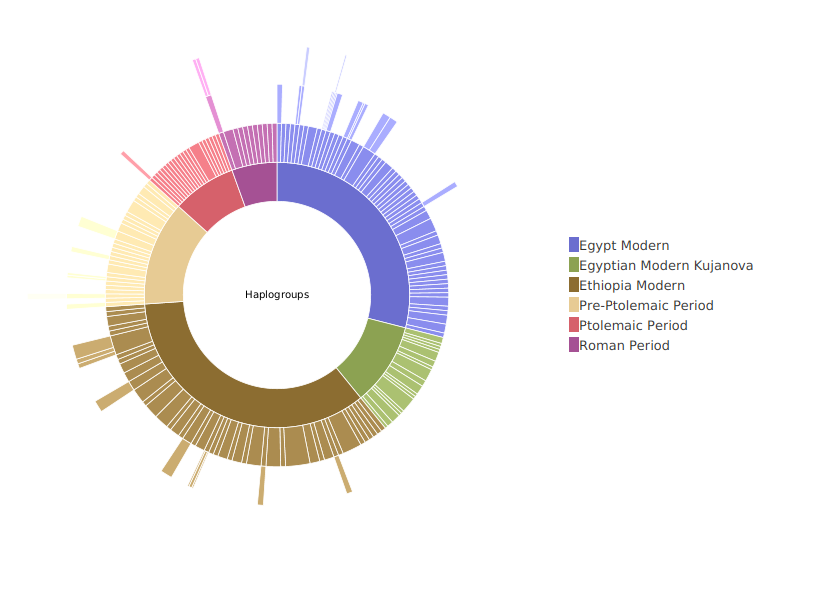
\includegraphics[width=0.8\textwidth]{imagesBench/sunburst.png}
	\end{center}
\end{frame}




\begin{frame}
	\frametitle{mitobench: Current visualization methods}
	\begin{itemize}
		\item Groups are represented as line
		\item Table rows are linked to corresponding lines in profile plot
	\end{itemize}
	
	\begin{center}
		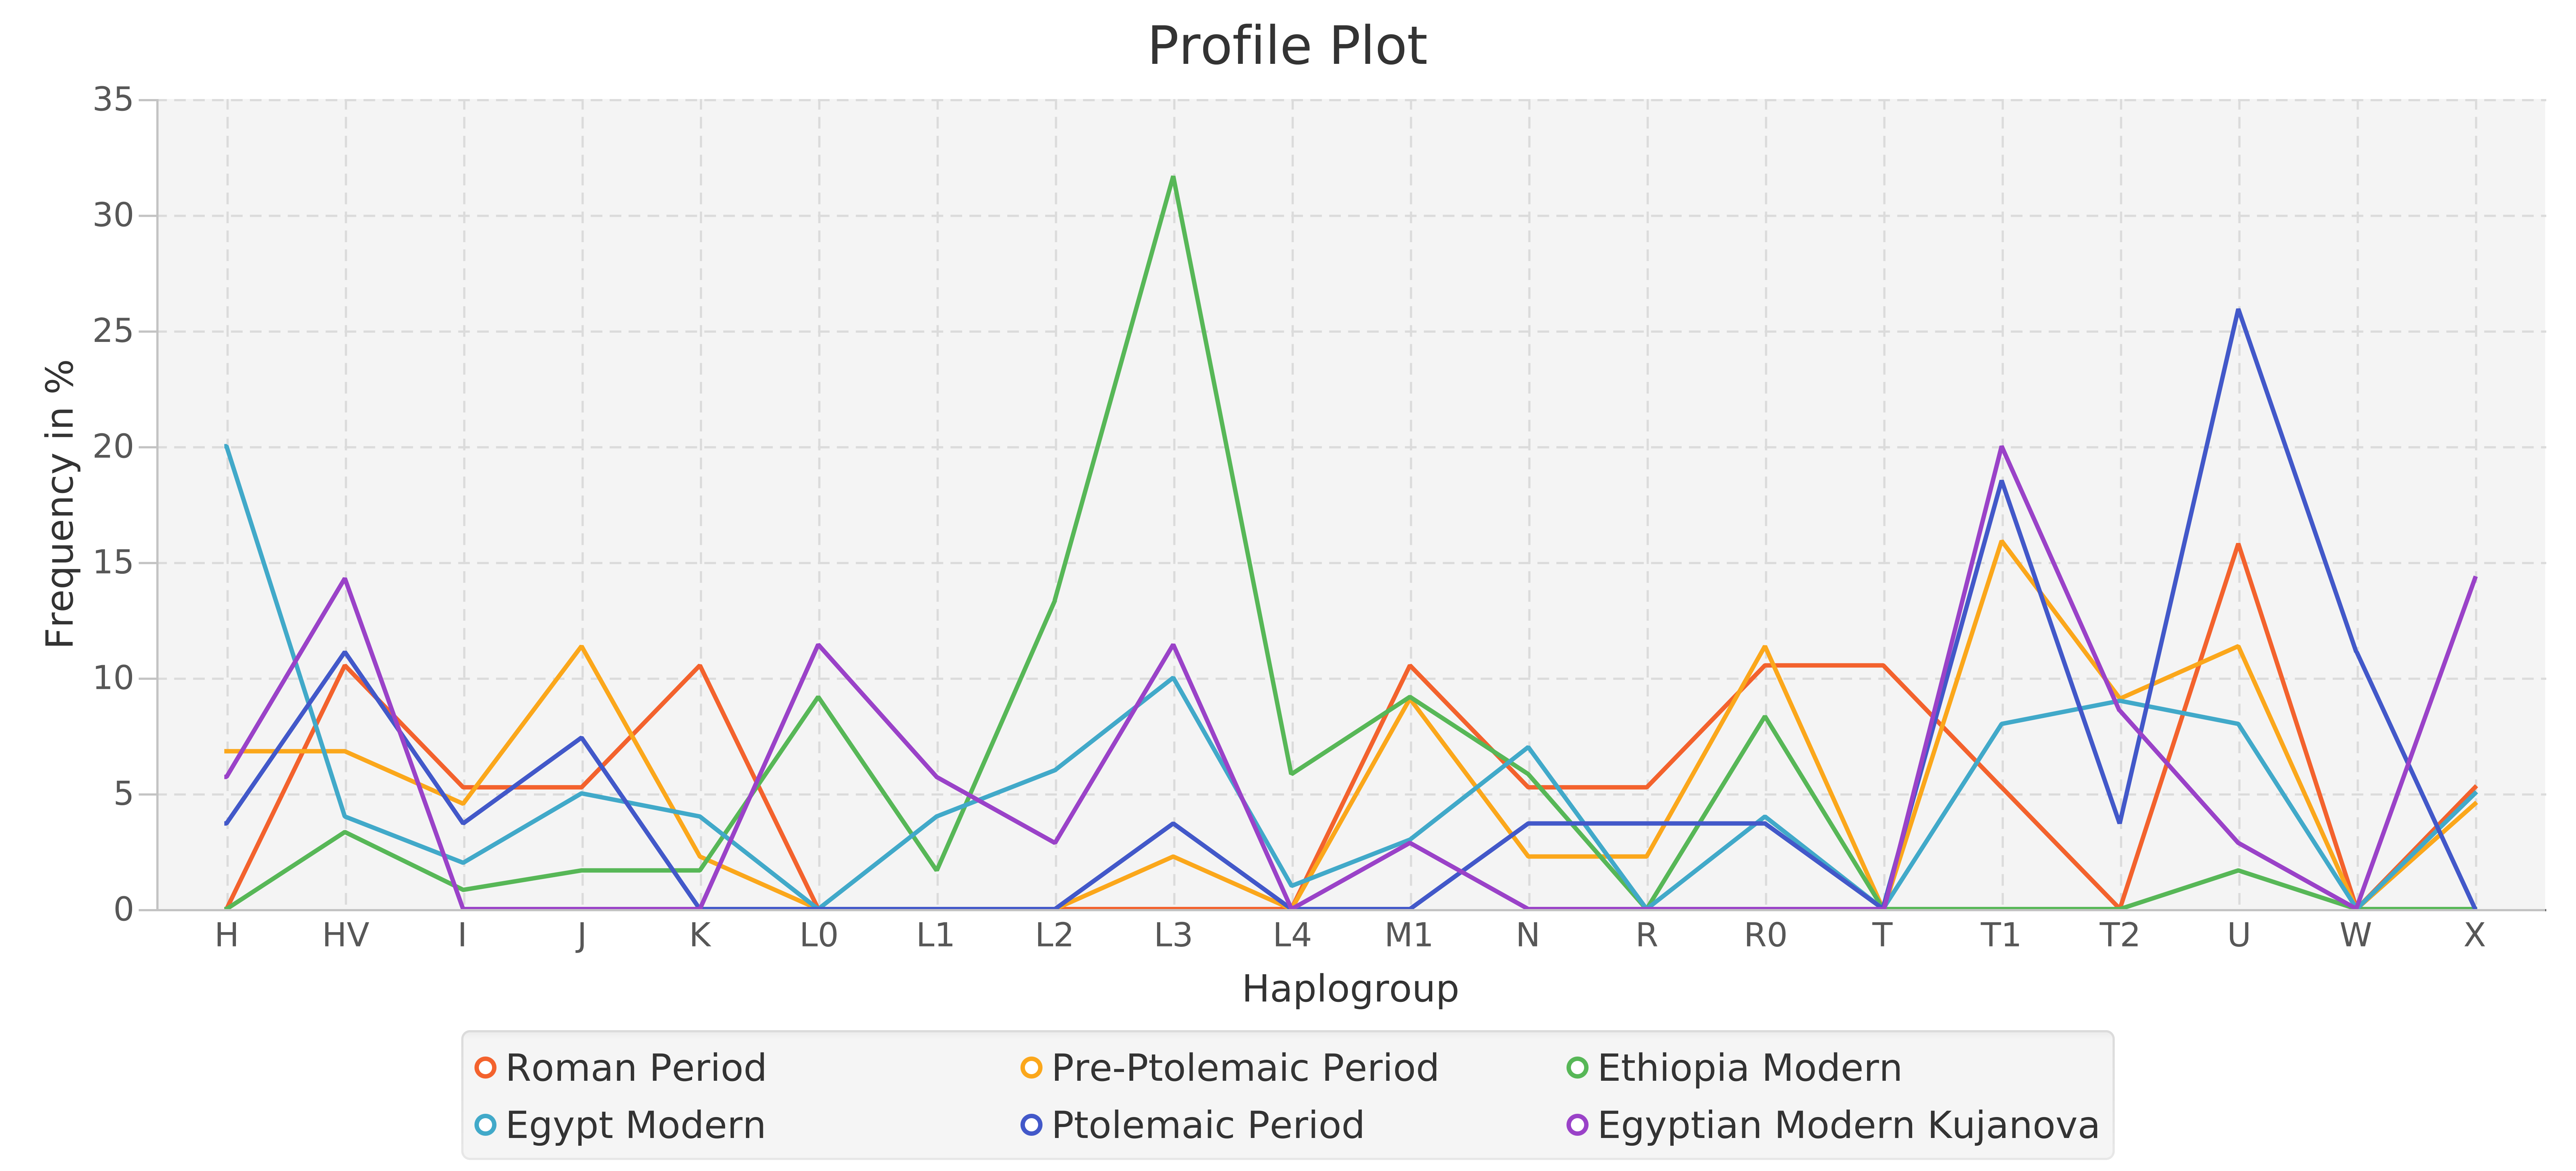
\includegraphics[width=0.8\textwidth]{imagesBench/profile.png}
	\end{center}
	\begin{center}
		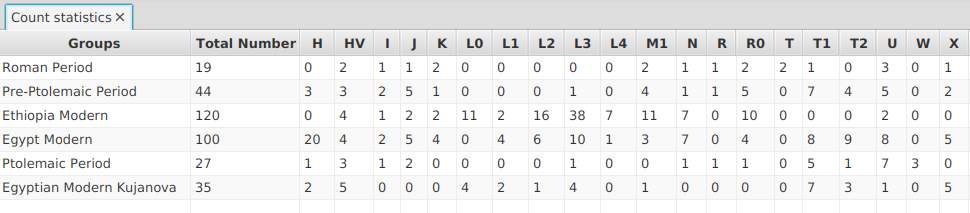
\includegraphics[width=0.7\textwidth]{imagesBench/profile_table.png}
	\end{center}
\end{frame}


\begin{frame}
\frametitle{mitoBench: Current visualization methods}
\begin{center}
	\includegraphics[width=\textwidth]{imagesBench/stackedBarchart.png}
	\end{center}
\end{frame}




%
%\begin{frame}
%\frametitle{mitoBench: Current visualization methods}
%\begin{center}
%		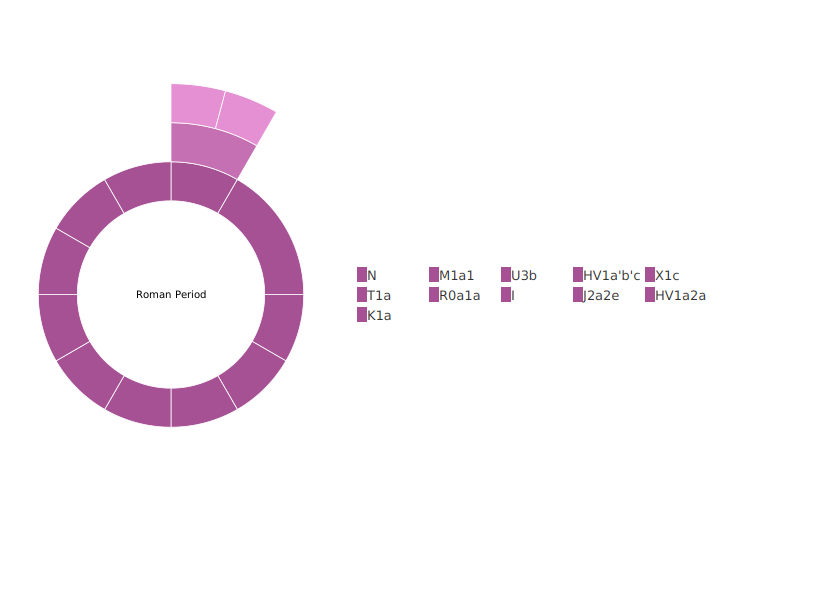
\includegraphics[width=0.7\textwidth]{imagesBench/sunburst_zoom.png}
%	\end{center}
%\end{frame}


\begin{frame}
\frametitle{mitoBench: Export Data and Figures}
\begin{center}
	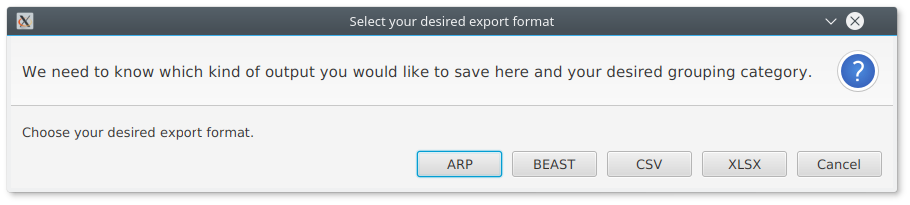
\includegraphics[width=0.7\textwidth]{imagesBench/exportData.png}
\end{center}

\begin{itemize}
	\item Export data into different file formats \\ 
    $\rightarrow$ input for downstream analysis tools
    \item Export figures 
\end{itemize}
\end{frame}


\begin{frame}
\frametitle{mitoBench: Export Project}
\begin{itemize}
\item Export whole project
	\begin{itemize}
		\item Export all table entries and grouping information \pause
        \item Restore a previously stored session with one click
	\end{itemize}
\end{itemize}
\end{frame}


%
%
%\begin{frame}
%Analysis with mitoBench:
%	\begin{itemize}
%		\item Easy and fast file conversions
%        \item Data exploration facilitated by visualizations
%        \item Data export: fast and less error-prone
%	\end{itemize}
%\end{frame}

\begin{frame}
\frametitle{mitoDB}
\begin{itemize}
\item Idea: Consolidate available data collections in a concise way
	\begin{itemize}
		\item Web-Frontend with Vaadin Java Framework
		\item Backend with PostgreSQL, providing sequence information and meta-data (SQL)
        \item Curated data upload with metadata
        \item Retrieval possible through WebUI and mitoBench
	\end{itemize}
\end{itemize}
\begin{figure}
\centering
    \begin{subfigure}[b]{0.3\textwidth}
        
\includegraphics[width=\textwidth]{imagesBench/postgresql.png}
    \end{subfigure}
    \qquad
    \begin{subfigure}[b]{0.3\textwidth}
        
\includegraphics[width=\textwidth]{imagesBench/vaadin.png}
    \end{subfigure}
\end{figure}
\end{frame}


\begin{frame}
\frametitle{mitoDB: Login}
\centering
	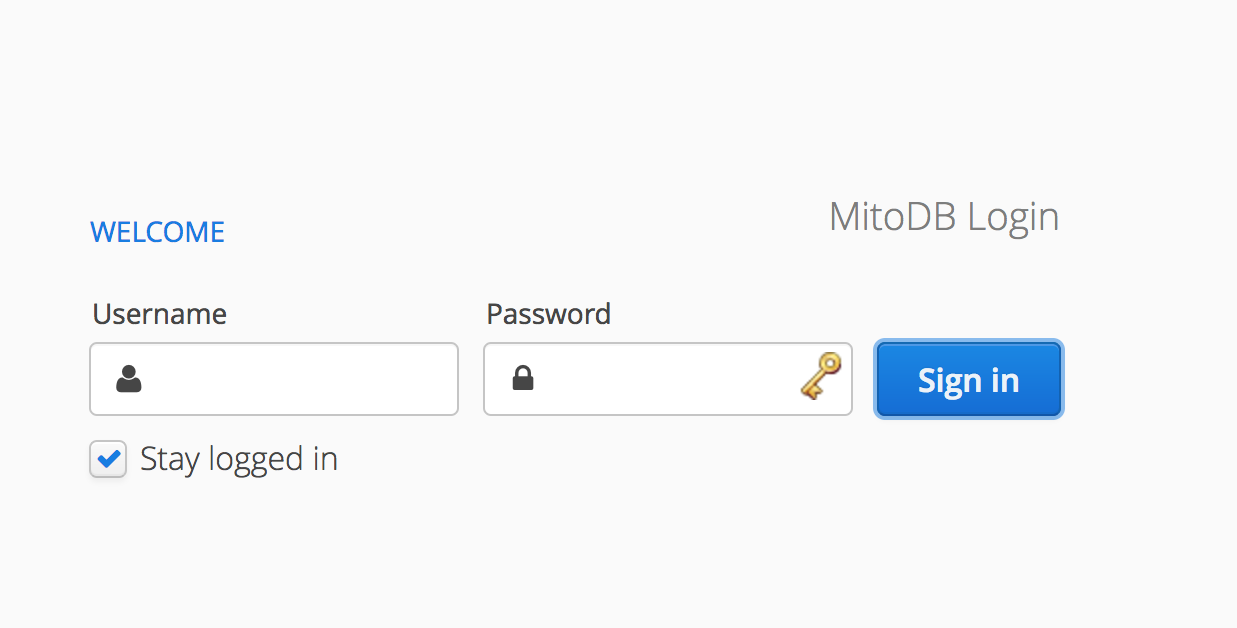
\includegraphics[scale=0.35]{imagesDB/mitodb_login.png}    
\begin{itemize}
\item Secure, encrypted login - registration will be available, too
\end{itemize}
\end{frame}

\begin{frame}
\frametitle{mitoDB: Dashboard}
\centering
	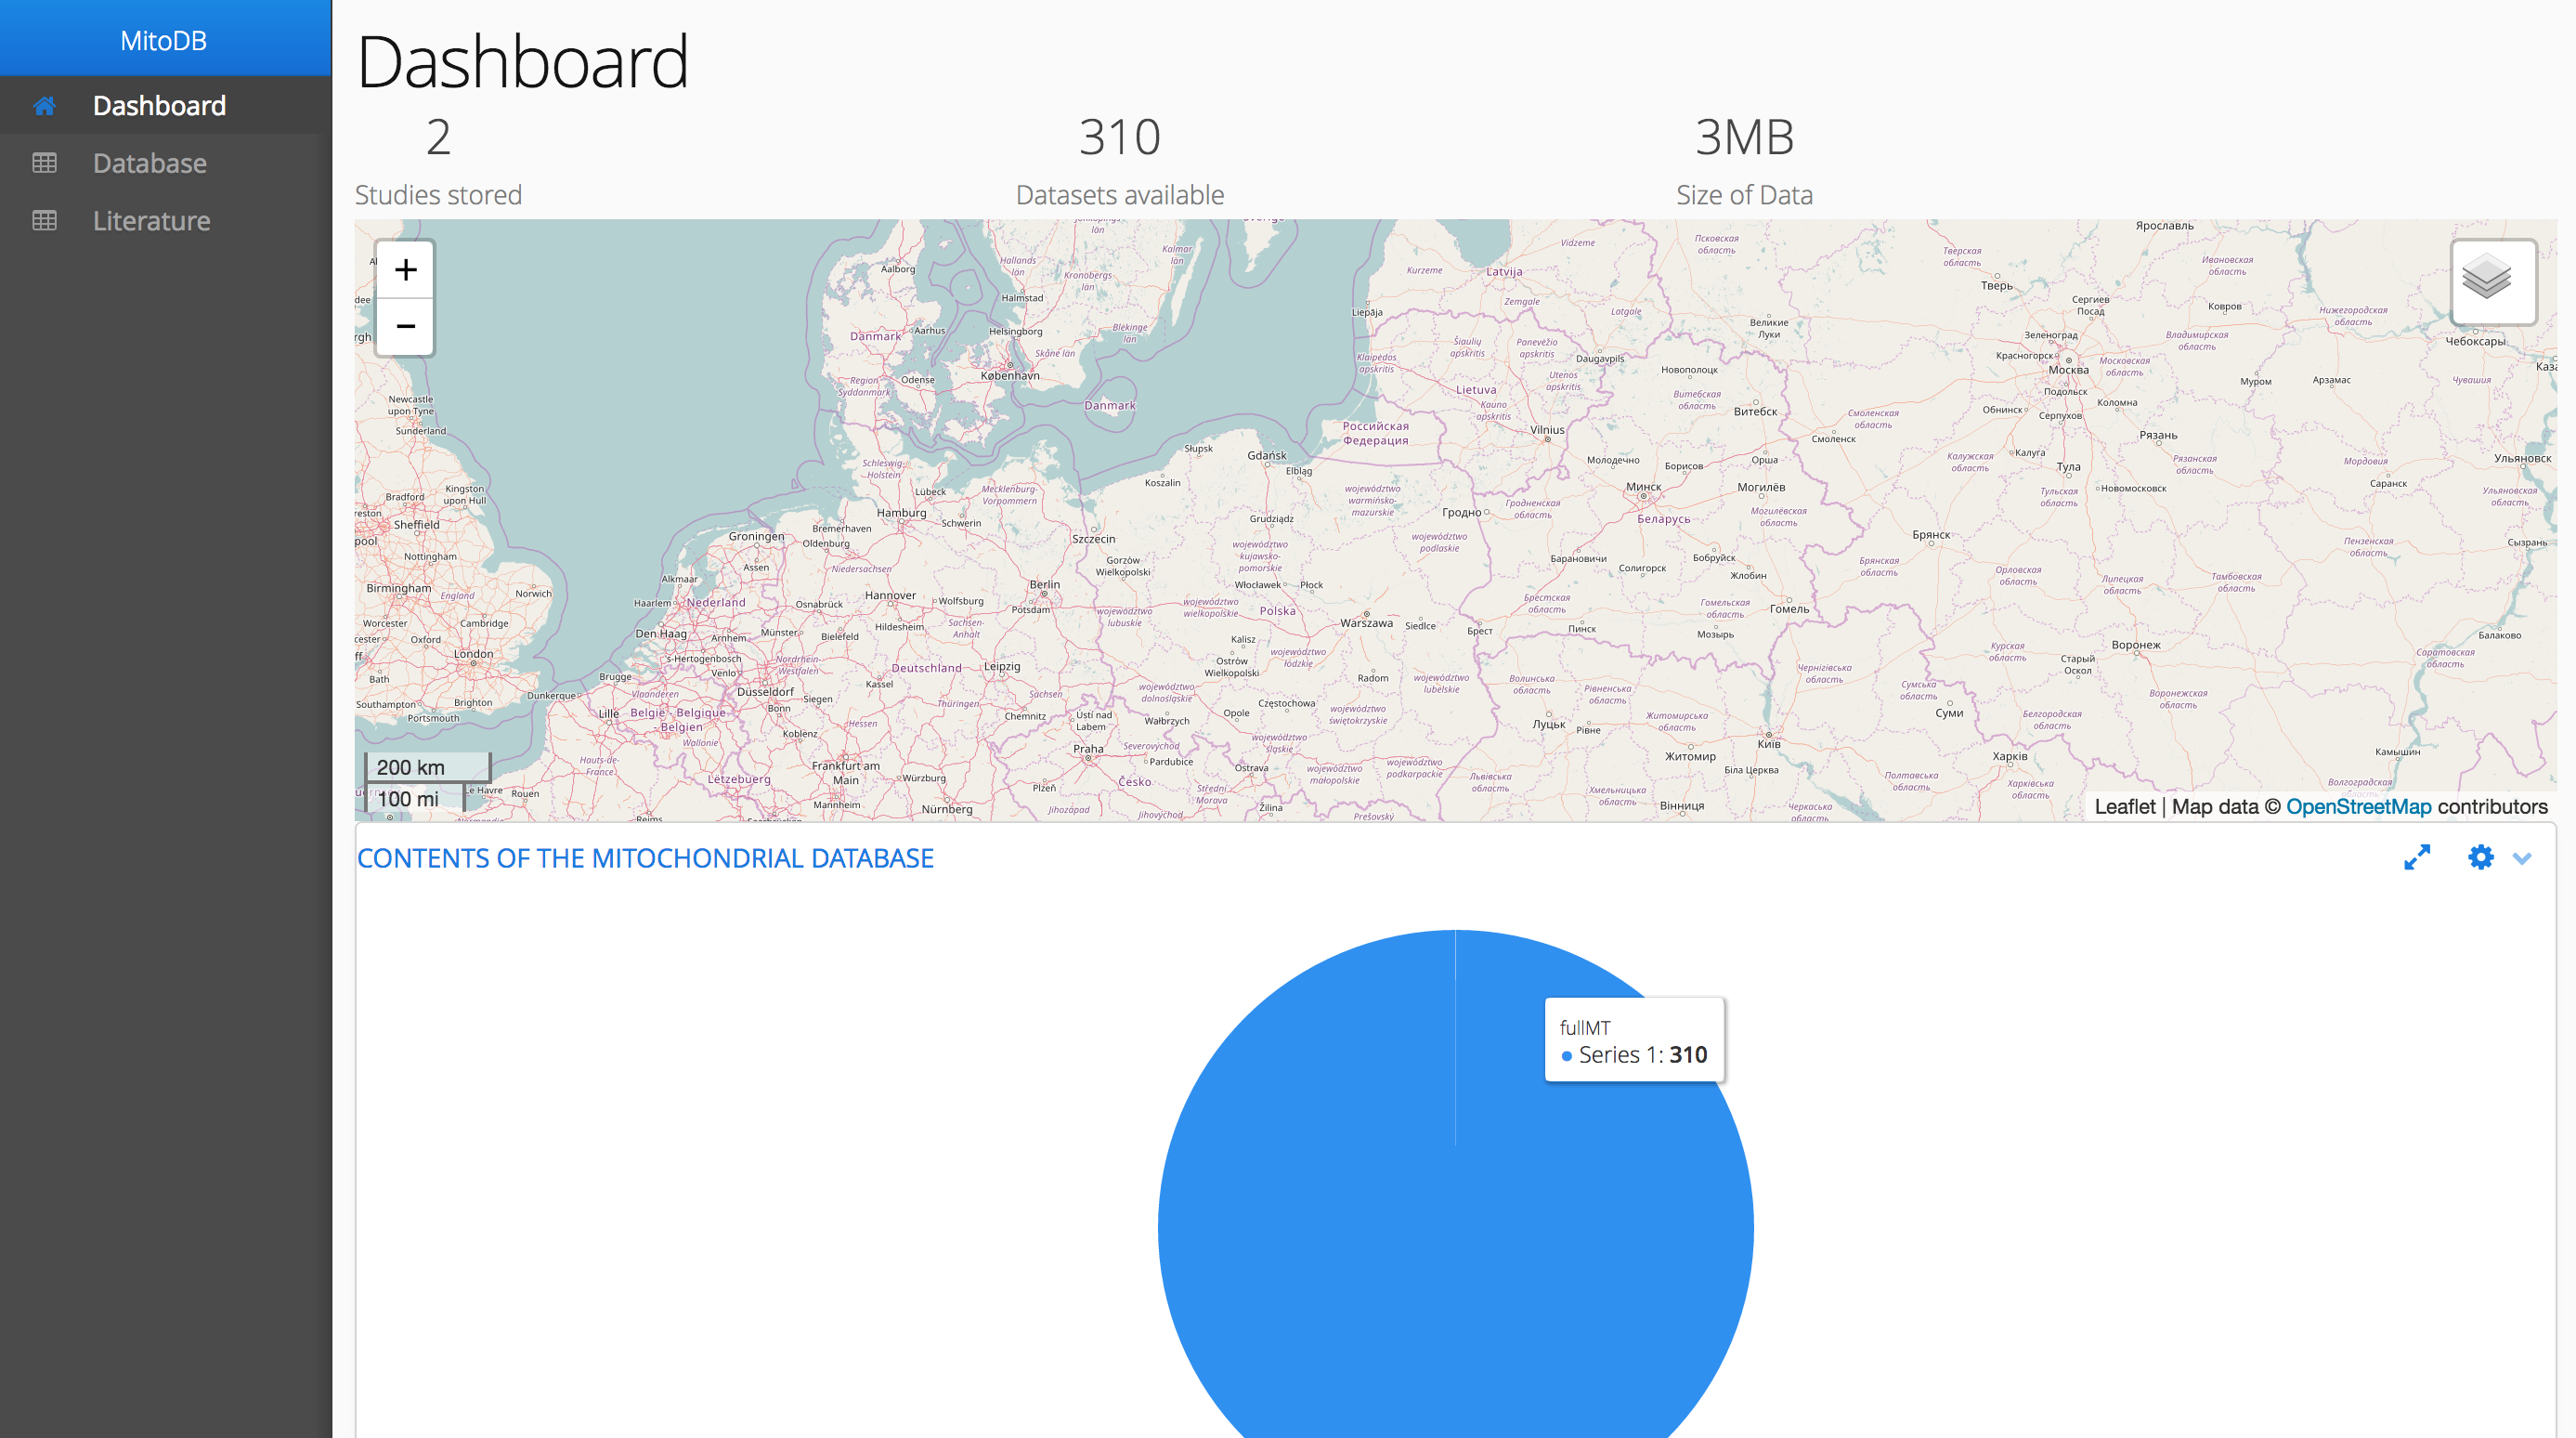
\includegraphics[scale=0.2]{imagesDB/mitodb_dashboard.png}
\begin{itemize}
\item Central `one stop shop` for database access
\item Left: Navigation, User Menu
\item Center: Map with geographic data points
\item Bottom: General information on the database (concept, not complete yet)
\end{itemize}
\end{frame}

\begin{frame}
\frametitle{mitoDB: DataTable}
\centering	
	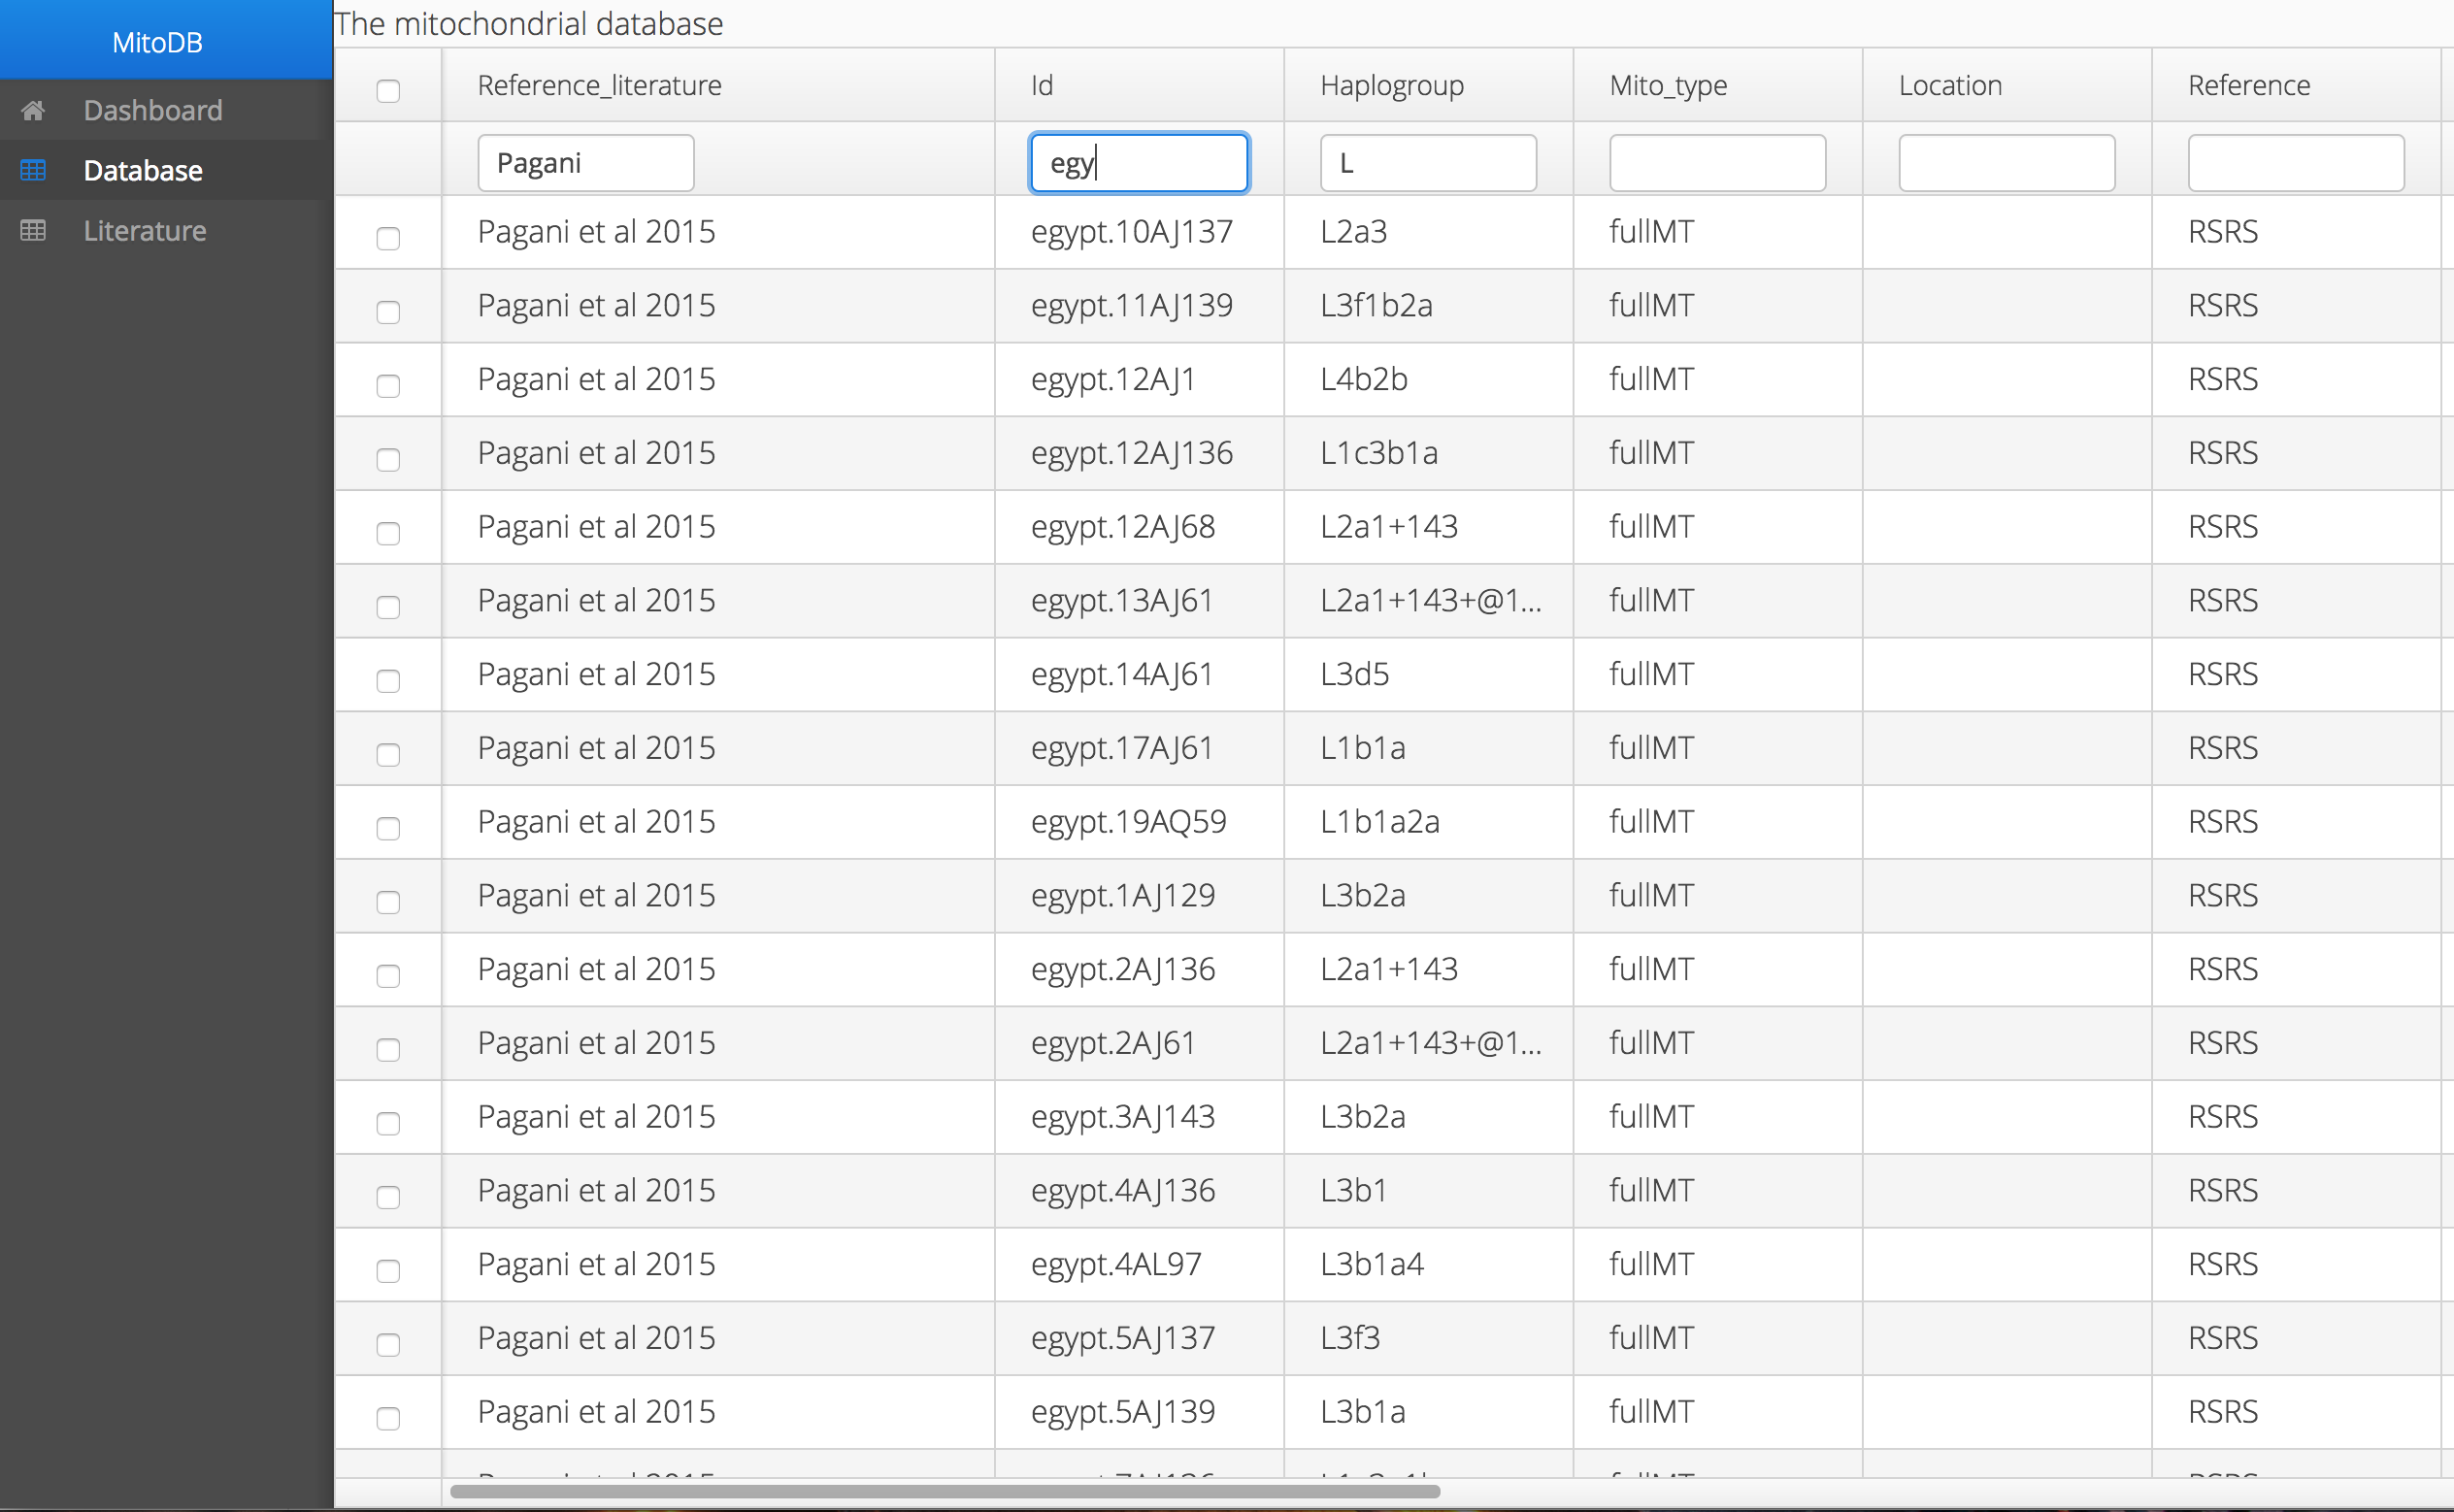
\includegraphics[scale=0.2]{imagesDB/mitodb_data.png}
\begin{itemize}
\item Data Table: Query functions, multiple selections, handle table data
\item  \textcolor{alexred}{Upcoming:} Export View: Drag and Drop selected data to different view
\end{itemize}
\end{frame}

\begin{frame}
\frametitle{mitoDB: References}
\centering
	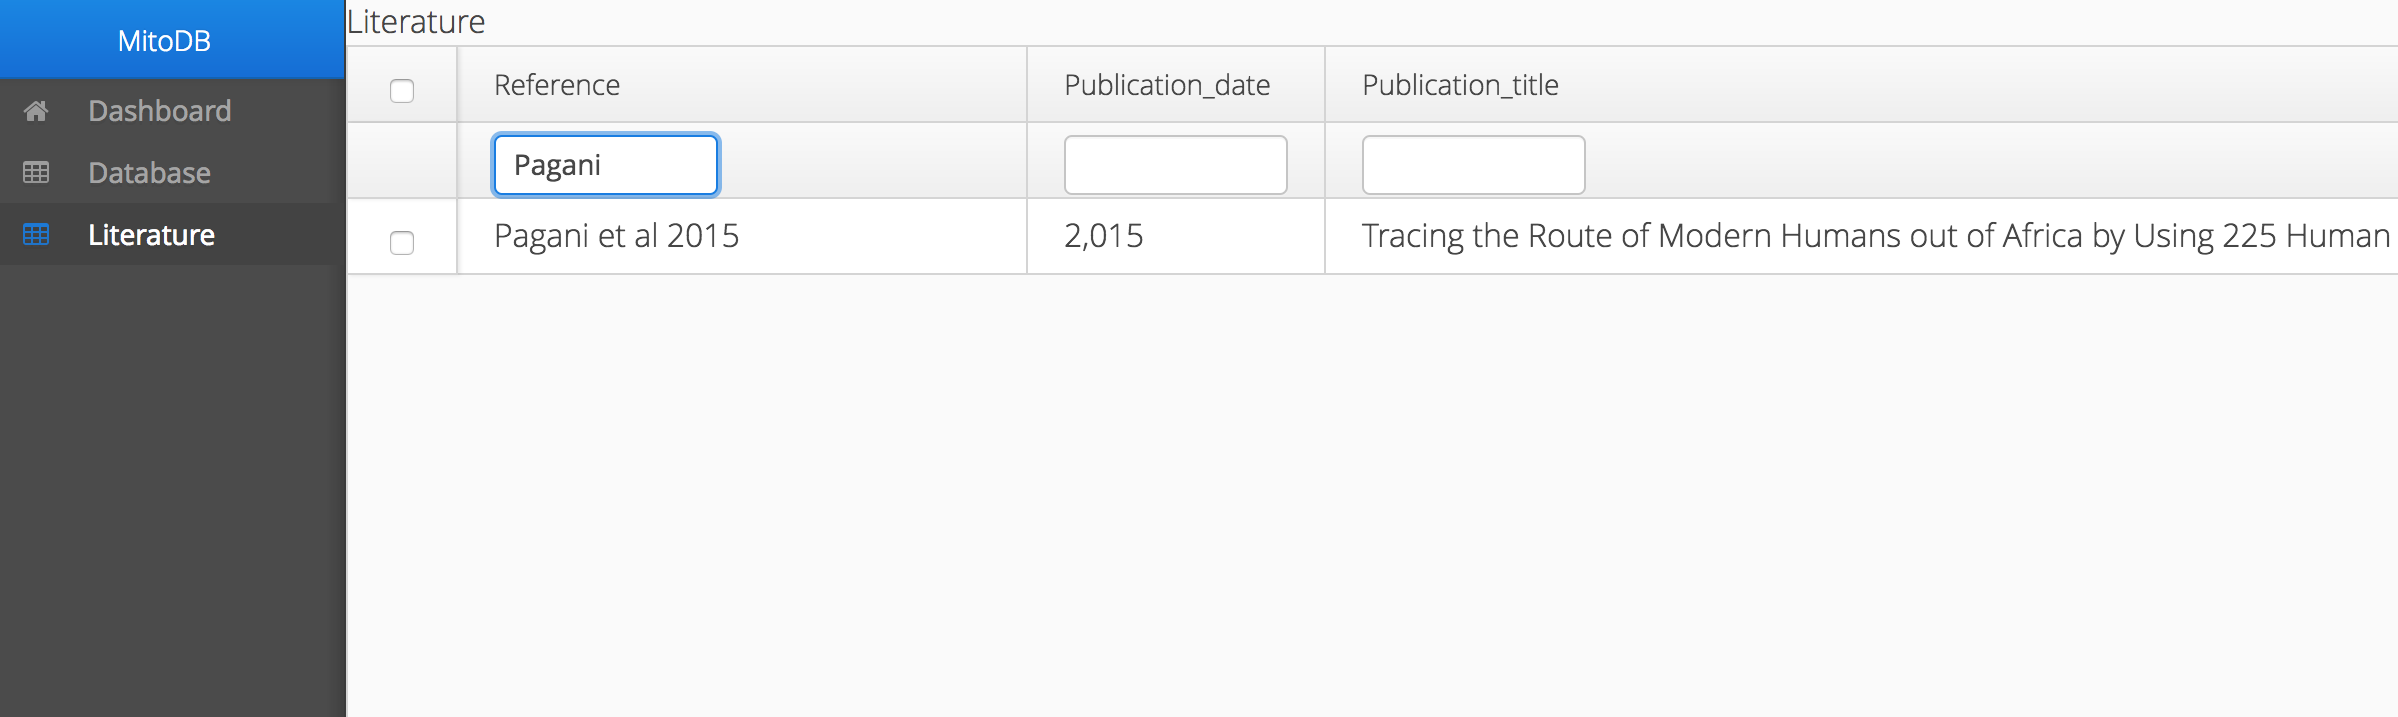
\includegraphics[scale=0.25]{imagesDB/mitodb_references.png}
\begin{itemize}
\item Literature database $\leftrightarrow$ Locked to samples (no inconsistencies)
\item Simple checking rules: No orphans - consistent updates 
\end{itemize}
\end{frame}

\begin{frame}
\frametitle{mitoDB: Prospects}
\centering
\begin{itemize}
\item Export Functionality: XLSX, ARP, BEAST, FastA, ... \pause
\item Import Functionality, with curation (upload, review mode) \pause
\item Data Access: Who can do what? Groups, Access Control etc. \pause
\item Workspace: Potentially some analysis inside the WebUI
\end{itemize}
\end{frame}



\begin{frame}
\frametitle{mitoBench: Prospects}
\begin{itemize}
\item Looking for early feedback/ideas:
\begin{itemize}
\item Data Manipulation: What can we do to improve further? 
\item Data Regulation: Curation, Access rights, Publication, $\ldots$
\end{itemize}
\end{itemize}
\end{frame}

\begin{frame}
\frametitle{Thank you}
\centering

\includegraphics[scale=0.1]{imagesBench/mitoBenchLogo.jpg}
\end{frame}

\end{document}

